% ============================================================
% RVT-Swarm: Recoverability-Aware Topology Control
% for Decentralized Swarm Formation
% ============================================================
\documentclass{ieeeaccess}
\pdfobjcompresslevel=0

\usepackage{cite}
\usepackage[utf8]{inputenc}
\usepackage[T1]{fontenc}
\usepackage{amsmath,amssymb,amsfonts,bm}
\usepackage{amsthm}
\usepackage{algorithm}
\usepackage{algorithmic}
\usepackage{textcomp}

\makeatletter
\AtBeginDocument{\DeclareMathVersion{bold}
\SetSymbolFont{operators}{bold}{T1}{times}{b}{n}
\SetSymbolFont{NewLetters}{bold}{T1}{times}{b}{it}
\SetMathAlphabet{\mathrm}{bold}{T1}{times}{b}{n}
\SetMathAlphabet{\mathit}{bold}{T1}{times}{b}{it}
\SetMathAlphabet{\mathbf}{bold}{T1}{times}{b}{n}
\SetMathAlphabet{\mathtt}{bold}{OT1}{pcr}{b}{n}
\SetSymbolFont{symbols}{bold}{OMS}{cmsy}{b}{n}
\renewcommand\boldmath{\@nomath\boldmath\mathversion{bold}}}
\makeatother
\makeatletter
\newcommand{\removelatexerror}{\let\@latex@error\@gobble}
\makeatother
\usepackage{graphicx}
\usepackage{float}
\usepackage{stfloats}
\usepackage{booktabs}
\usepackage{multirow}
\usepackage{xcolor}
\usepackage{pict2e}
\usepackage{hyperref}
\usepackage{cleveref}
\usepackage{pifont}
\newcommand{\cmark}{\ding{51}}
\newcommand{\xmark}{\ding{55}}
\newcommand{\pmark}{$\triangle$}
\newcommand{\na}{\textemdash}
\newsavebox{\ORCIDlogo}
\savebox{\ORCIDlogo}{%
\setlength{\unitlength}{\dimexpr 1em/256\relax}%
\begin{picture}(256,256)%
  \color[HTML]{A6CE39}\put(128,128){\circle*{256}}%
  \color{white}%
  \put(78.6,199.2){\circle*{20}}%
  \moveto(70.9,176)\lineto(86.3,176)\lineto(86.3,69.8)\lineto(70.9,69.8)%
  \closepath\fillpath%
  \moveto(108.9,176.9)\lineto(150.5,176.9)%
  \curveto(190.1,176.9)(207.5,148.6)(207.5,123.3)%
  \curveto(207.5,95.0)(186.0,69.7)(150.7,69.7)%
  \lineto(108.9,69.7)%
  \closepath\fillpath%
  \color[HTML]{A6CE39}%
  \moveto(124.3,83.6)\lineto(148.8,83.6)%
  \curveto(183.7,83.6)(191.7,110.1)(191.7,123.3)%
  \curveto(191.7,144.8)(178.0,163.0)(148.0,163.0)%
  \lineto(124.3,163.0)%
  \closepath\fillpath%
\end{picture}%
}
\newcommand{\orcidicon}[1]{\kern .08em\href{https://orcid.org/#1}{\usebox{\ORCIDlogo}}}

\DeclareMathOperator*{\argmax}{arg\,max}
\DeclareMathOperator*{\argmin}{arg\,min}
\newcommand{\R}{\mathbb{R}}
\newcommand{\cG}{\mathcal{G}}
\newcommand{\cN}{\mathcal{N}}
\newcommand{\cT}{\mathcal{T}}
\newcommand{\cS}{\mathcal{S}}
\newcommand{\bfu}{\mathbf{u}}
\newcommand{\bfp}{\mathbf{p}}
\newcommand{\bfv}{\mathbf{v}}
\newcommand{\bfe}{\mathbf{e}}

\begin{document}

\history{Date of publication xxxx 00, 0000, date of current version xxxx 00, 0000.}
\doi{10.1109/ACCESS.XXXX.XXXXXXX}

\title{RVT-Swarm: Recoverability-Aware Topology Control for Decentralized Swarm Formation}

\author{\uppercase{Dinh Duy Nguyen}\authorrefmark{1}\orcidicon{0009-0005-7812-9546}, \uppercase{Cuong Manh Hoang}\authorrefmark{1,2}\orcidicon{0009-0007-5207-1627}, \uppercase{Hieu Trung Nguyen}\authorrefmark{1}, and \uppercase{Hoang Anh Pham}\authorrefmark{1}\orcidicon{0000-0001-9621-9266}}


\address[1]{AViS Lab., Faculty of Electronics Engineering 1, Posts and Telecommunications Institute of Technology, Hanoi, Vietnam.}
\address[2]{Faculty of Information Technology, Posts and Telecommunications Institute of Technology, Hanoi, Vietnam.}

\markboth
{Duy \headeretal: RVT-Swarm: Recoverability-Aware Topology Control for Decentralized Swarm Formation}
{Duy \headeretal: RVT-Swarm: Recoverability-Aware Topology Control for Decentralized Swarm Formation}

\corresp{Corresponding author: Hoang Anh Pham (email: anhph@ptit.edu.vn).}

\titlepgskip=-15pt


\begin{abstract}
Decentralized swarm control scales well and avoids a single point of
failure. The main difficulty appears in cluttered environments. Under
local sensing, a swarm must do more than avoid immediate collisions. It
must also preserve a useful formation, pass through bottlenecks, and
regroup after deformation. In this paper, we propose Recoverability-Aware Topology Control
(RVT-Swarm), a decentralized graph controller that selects both
continuous robot actions and a discrete formation topology from a small
candidate set. Given a local interaction graph, the model predicts a
topology-conditioned action bank together with a recoverability score
map that estimates whether each candidate topology can support safe
progress and return to the desired formation. During training,
counterfactual rollouts supervise the action bank, topology preference,
recoverability map, and auxiliary context heads of a multi-head graph
network. During execution, the recoverability map guides topology
selection, formation-geometry updates, and a lightweight safety
projection. In the reported benchmark, RVT-Swarm achieves the strongest
overall performance among the compared methods. These results indicate
that explicit recoverability reasoning improves decentralized swarm
formation in clutter while remaining competitive with stronger reactive
safety filters on instantaneous safety.
\end{abstract}

\begin{keywords}
Multi-robot systems, swarm robotics, formation control, graph neural networks, multi-agent systems, and autonomous navigation.
\end{keywords}

\maketitle


\section{Introduction}
\label{sec:intro}

Multi-robot formations are useful when they remain both
\emph{safe} and \emph{task-capable}. In warehouse logistics,
cooperative inspection, and search-and-rescue, a team must do more than
avoid collisions. It must also keep enough structure to pass through
clutter, regroup, and keep moving toward a common goal. Garg
et al.~\cite{garg2024safe_multirobot_review}, Deng
et al.~\cite{deng2024formation_adaptation}, and Xie
et al.~\cite{xie2025multi_uav_formation_rl} all highlight this need.
The problem becomes harder in decentralized settings with only local
sensing, as illustrated by the contrast in \Cref{fig:teaser}.

\begin{figure}[!t]
\centering
\begin{minipage}[t]{0.49\columnwidth}
\centering
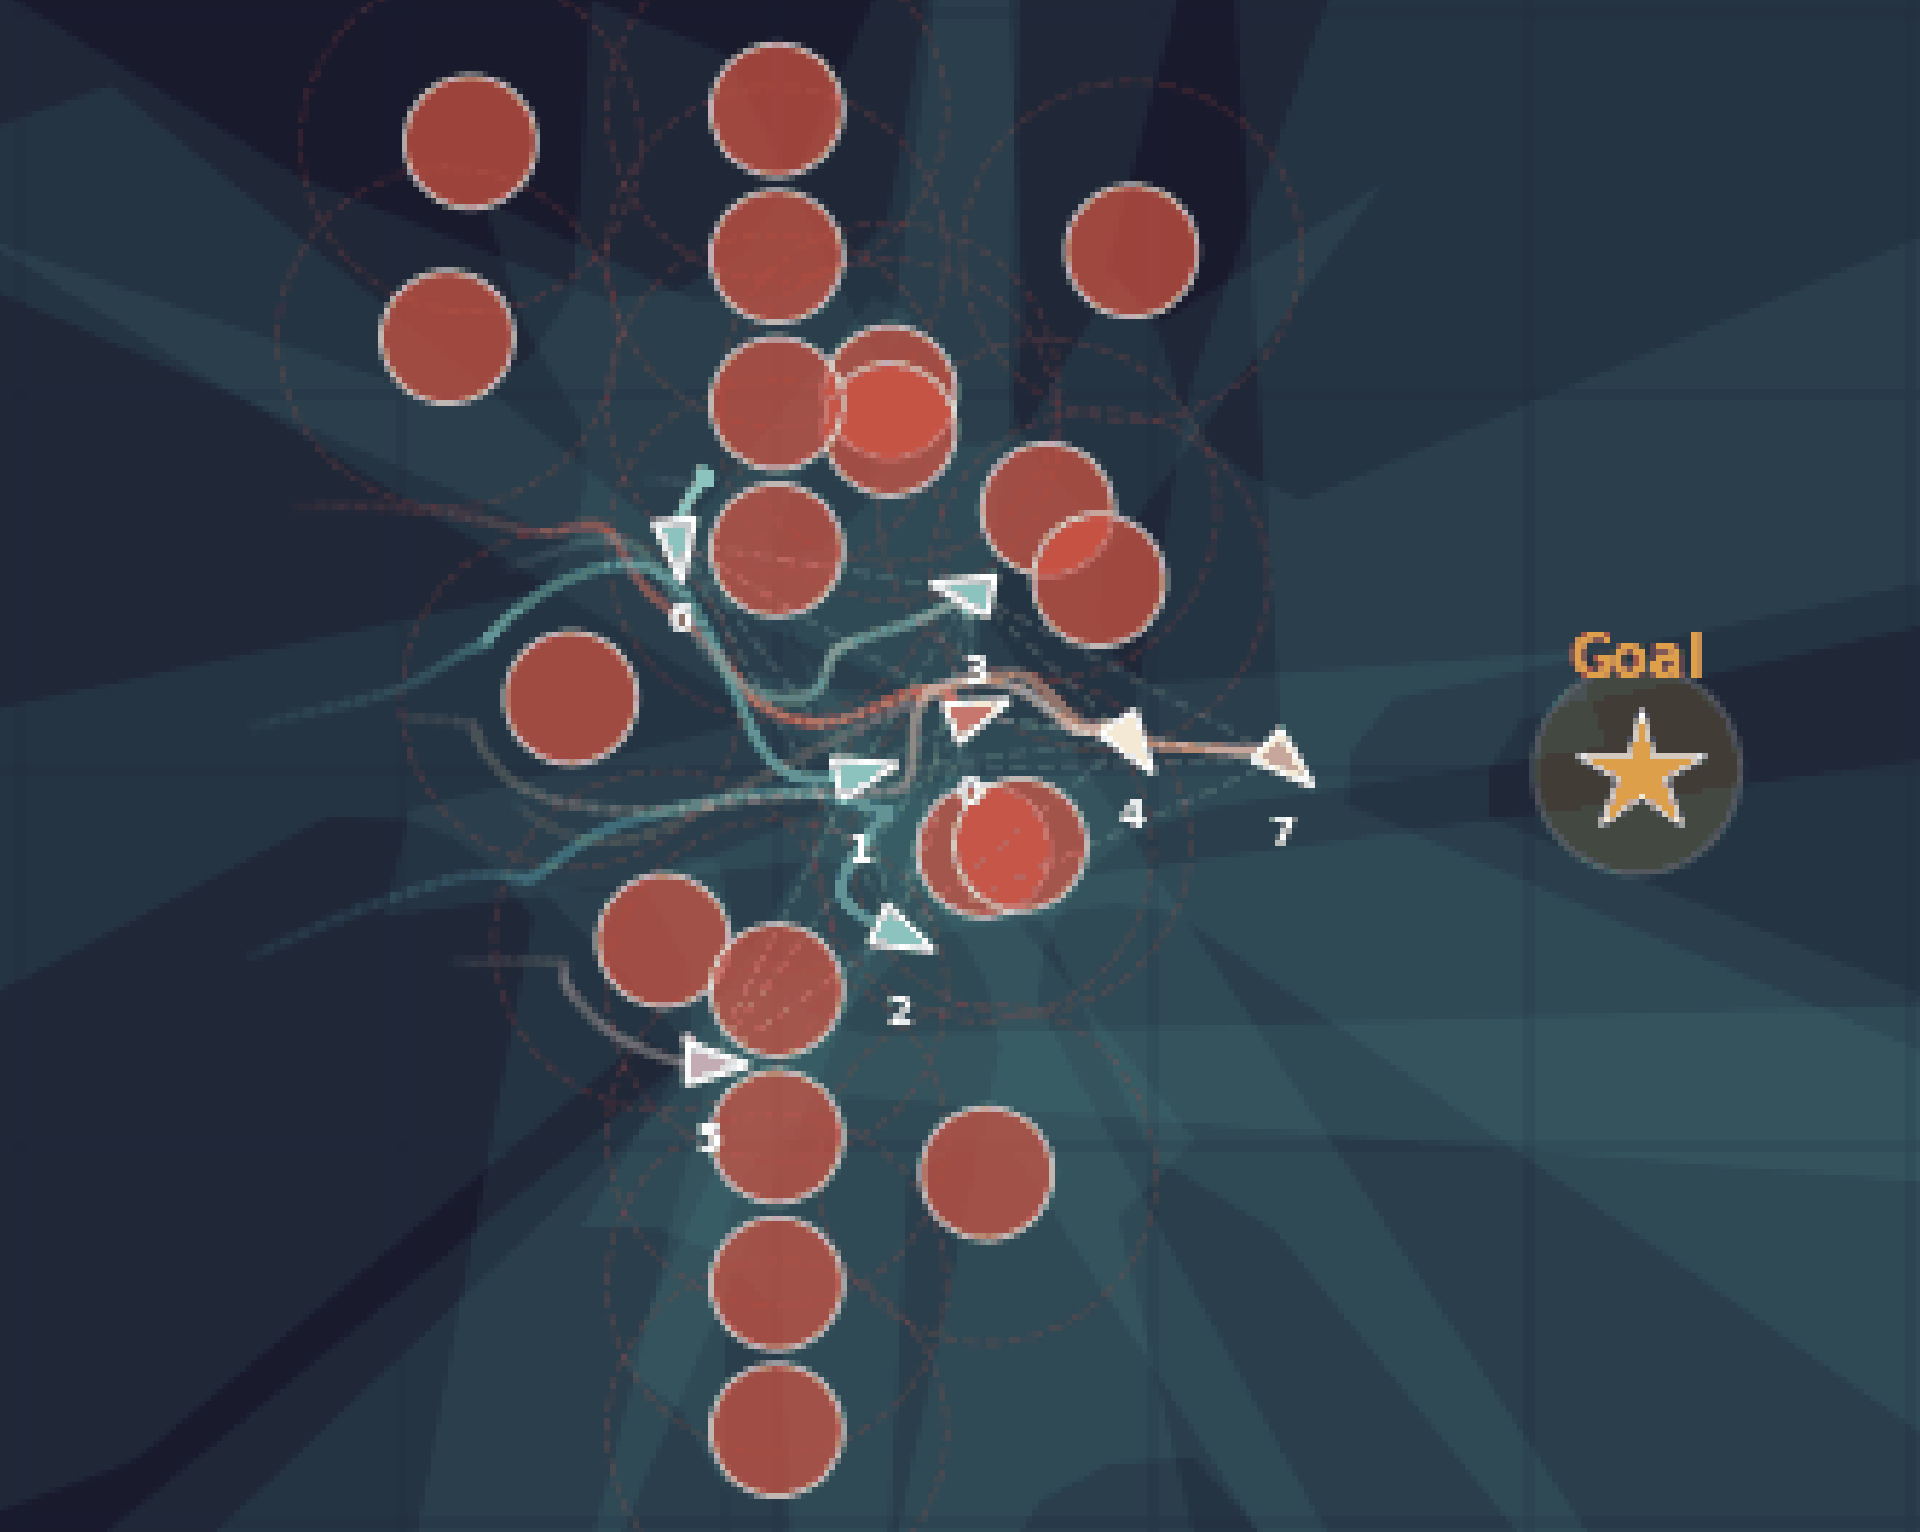
\includegraphics[width=\linewidth]{figures/teaser/b.png}
\par\vspace{1mm}
{\footnotesize\textbf{(a) Without Recovery}}
\end{minipage}
\hfill
\begin{minipage}[t]{0.49\columnwidth}
\centering
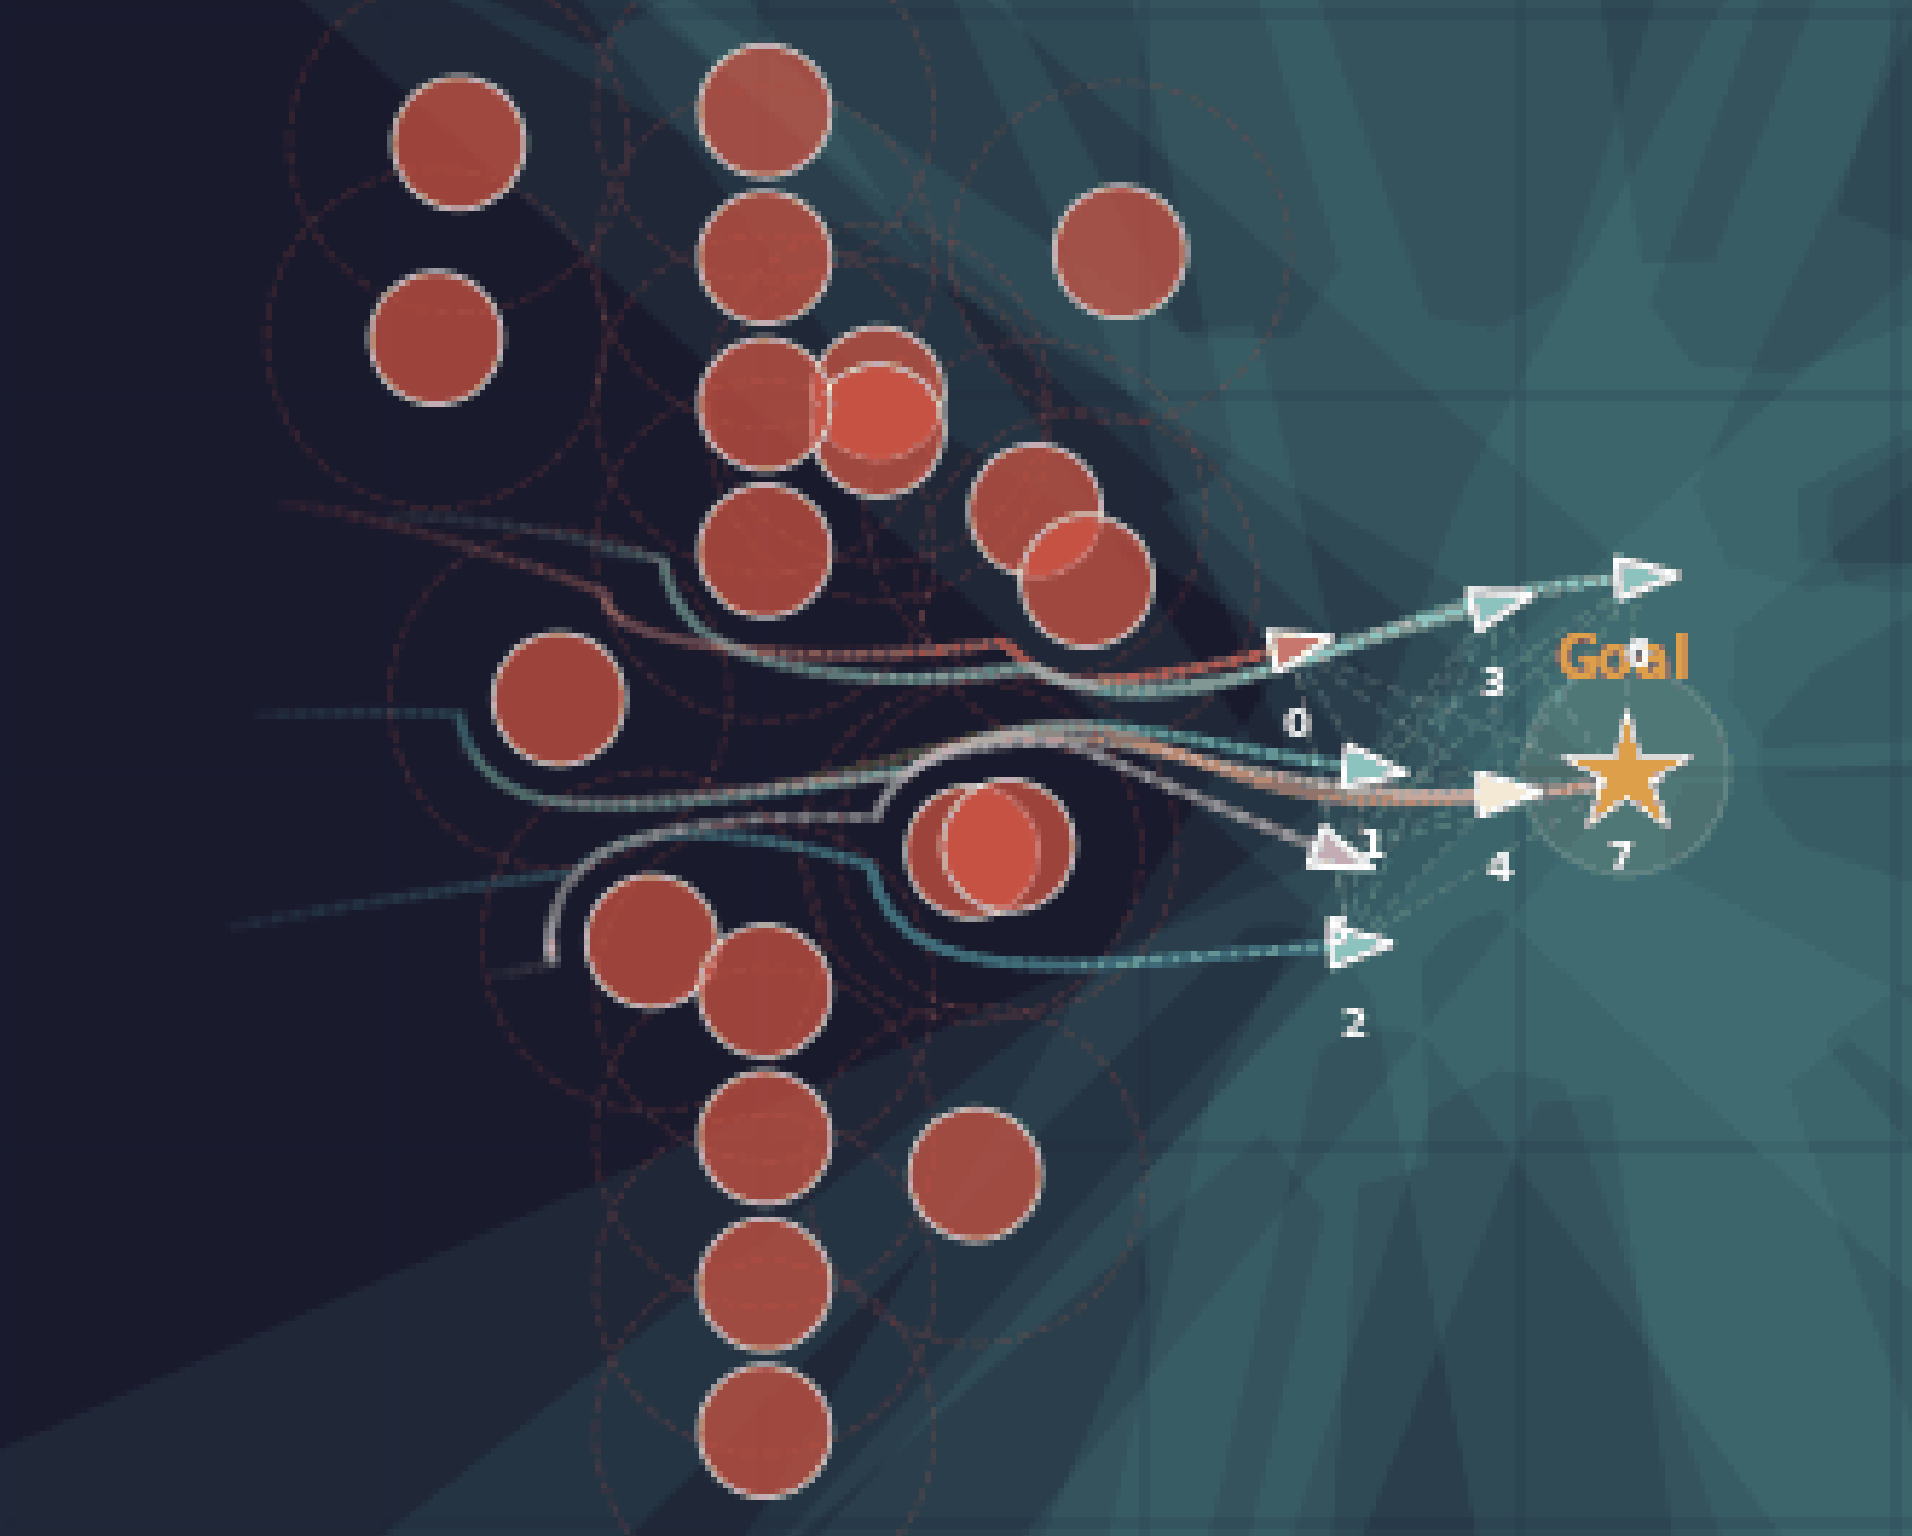
\includegraphics[width=\linewidth]{figures/teaser/a.png}
\par\vspace{1mm}
{\footnotesize\textbf{(b) With Recovery}}
\end{minipage}
\caption{Effect of recoverability-aware topology reasoning in a cluttered bottleneck. From the same shared local input, controllers without an explicit recoverability signal preserve a less useful formation structure, whereas RVT-Swarm selects a recoverable structural response that opens a clearer path toward the goal. In the teaser, triangular markers denote UGVs, red circles denote obstacles, and the star labeled \textit{goal} denotes the target.}
\label{fig:teaser}
\end{figure}

Existing approaches usually solve only part of this problem.
Graph-based decentralized controllers scale well to large teams, but
they often map local observations directly to motion and do not model
whether the team can still \emph{recover} a useful formation after
local reconfiguration. Examples include Zhou
et al.~\cite{muthusamy2024gnn_generalizability} and Goeckner
et al.'s \emph{MAGEC}~\cite{goeckner2024magec}. Control-barrier-function
(CBF) methods, such as \emph{GCBF+}~\cite{zhang2025gcbf_plus}, Butler
et al.~\cite{butler2024collaborative_safety}, and
\emph{DGPPO}~\cite{zhang2025dgppo}, provide strong instantaneous safety.
However, they focus on collision avoidance rather than return to a
formation tube. Adaptive-formation methods can change shape to fit the
environment, but they usually rely on hand-designed switching logic or implicit
policies without an explicit recoverability score over candidate
topologies, as in Deng
et al.~\cite{deng2024formation_adaptation} and Xie
et al.~\cite{xie2025multi_uav_formation_rl}. Reactive methods such as
ORCA~\cite{van2011orca} can keep the team moving, but often sacrifice
formation quality.

This paper takes a different view: instead of asking only whether the
current action is safe, we ask whether the current local state is
\emph{recoverable} under a small set of candidate topologies. In
RVT-Swarm, each local graph observation is mapped to a
topology-conditioned action bank, graph-level topology evidence, and a
recoverability score map. The controller then compares these topologies
counterfactually and applies a fixed rule based on recoverability,
keep/stay preference, uncertainty, context, and switching readiness. An
optional projection shield intervenes only when risk is high or when
all candidate topologies look unrecoverable.

The method does not claim an exact viability kernel or a formal
distributed reachability proof. Instead, it learns a short-horizon
surrogate of recoverability from counterfactual rollouts and uses that
surrogate online for topology adaptation. Runtime selection is
recoverability-first, while graph-level topology logits remain mainly a
fallback signal.

The method has two coupled stages. During training, counterfactual
rollout-score vectors are distilled into topology-conditioned action
targets, soft topology distributions, recoverability score maps, and
auxiliary context targets, so the network learns both what action to
take and how candidate topologies compare. During inference, the
learned score map drives topology selection, latent-geometry updates,
and a risk-triggered projection shield.

We make the following contributions:
\begin{enumerate}
    \item We introduce \emph{RVT-Swarm}, a decentralized framework for recoverability-aware topology control in swarm formation. Instead of treating topology change as a heuristic post-processing step or reducing safety to instantaneous collision avoidance, RVT-Swarm treats structural topology as an explicit online decision variable scored by short-horizon recoverability.

    \item We develop a rollout-supervised multi-head graph controller that learns this recoverability structure directly from counterfactual topology rollouts. The resulting Recoverability Field Network distills each sampled state into topology-conditioned action targets, soft topology distributions, recoverability score maps, uncertainty estimates, and auxiliary graph-level context, enabling the policy to learn not only what action to take but also which candidate topology remains most recoverable.

    \item We develop a recoverability-first inference stack in which graph-level topology evidence, recoverability scores, uncertainty, and auxiliary context are combined to choose a structural topology, select the corresponding action slice from a topology-conditioned action bank, update latent formation geometry, and invoke a progress-preserving shield only when risk is elevated.

    \item Across the reported benchmark, RVT-Swarm achieves the strongest overall performance among the compared methods, supporting the case for recoverability-aware topology control as a practical advantage for decentralized swarm formation.
\end{enumerate}

\section{Related Work}
\label{sec:related}

Table~\ref{tab:comparison} summarises the positioning of RVT-Swarm relative to the most relevant prior work families for our setting.

\begin{table*}[!t]
\centering
\caption{Positioning of RVT-Swarm relative to representative recent prior work.
\cmark~= primary capability; \pmark~= partially addressed;
\xmark~= not addressed. The table is intended as a qualitative
positioning summary for this work, rather than an exhaustive
taxonomy.}
\label{tab:comparison}
\scriptsize
\setlength{\tabcolsep}{4pt}
\renewcommand{\arraystretch}{1.12}
\begin{tabular}{lcc ccccccc}
\toprule
\textbf{Method} & \textbf{Venue} & \textbf{Year}
& \parbox[c]{0.09\textwidth}{\centering\textbf{Local graph}\\\textbf{distributed}}
& \parbox[c]{0.08\textwidth}{\centering\textbf{Formation}\\\textbf{aware}}
& \parbox[c]{0.09\textwidth}{\centering\textbf{Obstacle}\\\textbf{dynamics}}
& \parbox[c]{0.09\textwidth}{\centering\textbf{Topology}\\\textbf{adaptation}}
& \parbox[c]{0.09\textwidth}{\centering\textbf{Recoverability}\\\textbf{model}}
& \parbox[c]{0.10\textwidth}{\centering\textbf{Counterfactual}\\\textbf{selection}}
& \parbox[c]{0.08\textwidth}{\centering\textbf{Progress}\\\textbf{shield}} \\
\midrule
HJ safety/liveness~\cite{borquez2024hj_filtering}
    & T-RO & 2024 & \xmark & \xmark & \cmark
    & \xmark & \cmark & \xmark & \cmark \\
Belief-prop.\ MPC~\cite{jiang2024belief_mpc_formation}
    & RA-L & 2024 & \cmark & \cmark & \pmark
    & \pmark & \xmark & \xmark & \xmark \\
Robust MADER~\cite{kondo2024robust_mader}
    & RA-L & 2024 & \cmark & \pmark & \cmark
    & \xmark & \xmark & \xmark & \xmark \\
Cert.\ Reach.~\cite{li2025certifiable_reachability}
    & RA-L & 2025 & \pmark & \xmark & \cmark
    & \xmark & \cmark & \xmark & \xmark \\
DGPPO~\cite{zhang2025dgppo}
    & ICLR & 2025 & \cmark & \xmark & \cmark
    & \xmark & \xmark & \xmark & \cmark \\
GCBF+~\cite{zhang2025gcbf_plus}
    & T-RO & 2025 & \cmark & \pmark & \cmark
    & \xmark & \xmark & \xmark & \pmark \\
Goal-conv.\ swarm~\cite{park2025goal_convergence}
    & IJRR & 2025 & \cmark & \pmark & \cmark
    & \xmark & \xmark & \xmark & \xmark \\
RAIL~\cite{jung2025rail}
    & ICRA & 2025 & \pmark & \xmark & \cmark
    & \xmark & \cmark & \xmark & \xmark \\
Multi-UAV RL~\cite{xie2025multi_uav_formation_rl}
    & IROS & 2025 & \cmark & \cmark & \cmark
    & \pmark & \xmark & \xmark & \xmark \\
\midrule
\textbf{RVT-Swarm (ours)}
    & --- & 2026 & \cmark & \cmark & \cmark
    & \cmark & \cmark & \cmark & \cmark \\
\bottomrule
\end{tabular}
\end{table*}

\subsection{Decentralized Graph Policies}
Recent decentralised graph-policy work shows a clear progression toward using local message passing as the core inductive bias for scalable swarm control. Gama et al.~\cite{gama2022gnn_synthesis} formulate decentralised controller synthesis through graph neural networks and imitation learning, and Shi et al.'s \emph{Neural-Swarm2}~\cite{shi2022neural_swarm2} demonstrates that learned interaction models can support heterogeneous multirotor teams. Later work becomes more task-driven: \emph{MAGEC}~\cite{goeckner2024magec} emphasises resilient graph-based coordination, and \emph{Learning Decentralised Multi-Robot PointGoal Navigation}~\cite{soualhi2025pointgoal} extends the same local-policy paradigm to decentralised navigation in clutter. The progression is important because the later systems become more realistic and navigation-oriented. Yet, they still treat the graph policy primarily as a direct mapping from local observations to actions or coordination signals. RVT-Swarm remains in this decentralised graph-policy regime, but departs from it by explicitly evaluating candidate team topologies and selecting among them online through a topology-conditioned recoverability map.

\subsection{Safety-Critical Multi-Robot Control}
Safety-critical multi-robot control has followed a similar progression from analytical safety refinement to learned distributed safety policies. Tonkens and Herbert~\cite{tonkens2022refining_cbf_hj} show that Hamilton--Jacobi analysis can sharpen barrier-based control rather than merely wrap around it. Subsequent work broadens this perspective: Garg et al.~\cite{garg2024safe_multirobot_review} synthesise the safe-learning design space for multi-robot systems, Borquez et al.~\cite{borquez2024hj_filtering} make safety and liveness filtering explicit through reachability reasoning, and Mestres et al.~\cite{mestres2024distributed_safe_navigation} provide a distributed CBF reference point for multi-agent navigation without an explicit topology-selection layer. More recent learned methods such as \emph{GCBF+}~\cite{zhang2025gcbf_plus} and \emph{DGPPO}~\cite{zhang2025dgppo} push this line toward scalable graph-structured safe control. RVT-Swarm is informed by this literature but differs in its emphasis: instead of solving a certified safety problem at every step, it uses a lightweight projection shield only after the recoverability network and the topology selector have chosen the most promising formation mode.

\subsection{Adaptive Formation and Recoverability}
Work on clutter-aware formation navigation has shifted from decentralised trajectory planning to richer models of coordination, uncertainty, and formation adaptation. \emph{MADER}~\cite{tordesillas2022mader} establishes decentralised multi-agent planning in dynamic environments, and \emph{AMSwarm}~\cite{adajania2023amswarm} brings that discussion closer to safe swarm motion in cluttered aerial settings. Later methods broaden the planning stack rather than merely repeating it: \emph{Robust MADER}~\cite{kondo2024robust_mader} adds delay robustness, distributed belief-propagation MPC~\cite{jiang2024belief_mpc_formation} introduces uncertainty-aware formation navigation, Stein variational belief propagation~\cite{pavlasek2024stein_belief} extends approximate-inference ideas to coordination. Assignment-free mean-shift formation~\cite{zhang2024mean_shift_shape} removes explicit target assignment from shape control. The most recent decentralised planners, including Park et al.~\cite{park2025goal_convergence} and Senbaslar et al.~\cite{senbaslar2025dream}, push further into cluttered, goal-directed swarm navigation, while RL-based formation-preserving obstacle avoidance~\cite{xie2025multi_uav_formation_rl} applies learning directly to the multi-UAV setting. RVT-Swarm is closest to this recent generation, but differs in treating topology change as an explicit online decision variable rather than as an emergent byproduct of a single optimiser or policy.

The recoverability side of RVT-Swarm is closer to recent reachability-informed safety learning than to classical fixed-formation control. Borquez et al.~\cite{borquez2024hj_filtering} use Hamilton--Jacobi reasoning to filter unsafe or non-progressing behaviour; Li et al.~\cite{li2025certifiable_reachability} push this direction toward learned certifiable reachability representations; and \emph{RAIL}~\cite{jung2025rail} combines reachability with imitation learning for safe execution. RVT-Swarm does not attempt to serve as a formal reachability engine. Instead, it learns a short-horizon recoverability surrogate that is cheap enough to evaluate for every candidate structural topology at runtime. Then it uses that surrogate to decide whether the team should keep its current structure, align into a line, or split into coordinated subteams before geometric intervention becomes necessary.

\section{Problem Setup}
\label{sec:problem}

\subsection{Environment, State, and Local Observation}
We consider $N$ robots moving in a 2D workspace with discrete-time
kinematics indexed by the step variable $k$,
\begin{equation}
\begin{aligned}
\bfp_i^{k+1} &= \bfp_i^k + \bfv_i^k\Delta t,\\
\bfv_i^{k+1} &= \bfv_i^k + \bfu_i^k\Delta t.
\end{aligned}
\label{eq:dynamics}
\end{equation}
Here $\bfp_i^k\in\R^2$ is the position of robot $i$ at step $k$,
$\bfv_i^k\in\R^2$ is its velocity, $\bfu_i^k\in\R^2$ is its control
input, and $\Delta t$ is the sampling period. The state and control
variables are continuous, but the evolution is observed and executed at
discrete steps. Speed and acceleration are bounded.

Let
\[
x_k=\bigl(\{\bfp_i^k,\bfv_i^k\}_{i=1}^N,\mathcal{O}_k\bigr)
\]
denote the joint swarm state, where $\mathcal{O}_k$ collects the
currently relevant obstacle states. The global state $x_k$ is useful
for writing the ideal control problem. However, the deployed policy does
not observe $x_k$ directly. Instead, robot $i$ receives a local
observation $o_i^k$, and the team-level observation is
$o_k=\{o_i^k\}_{i=1}^N$. Each $o_i^k$ is built from relative geometry,
obstacle context, goal direction, formation cues, and a local LiDAR
scan. The environment contains both static and dynamic obstacles,
including bottlenecked regions such as narrow passages.

\subsection{Topology-Conditioned Formation Objective}
The task is not only to reach the goal. The swarm must also preserve a
coherent formation while moving through clutter. A single fixed shape is
often not suitable everywhere. In open space, a compact two-dimensional
pattern is efficient. In a narrow corridor, the same pattern can block
progress. We therefore describe formation maintenance through a small
set of structural templates.

Let
\[
\bar{\bfp}^{\,k}=\frac{1}{N}\sum_{i=1}^N \bfp_i^k
\]
denote the swarm centroid at step $k$. For each candidate topology
$\tau\in\cT$, let
$\{\bm{\delta}_i^\tau\}_{i=1}^N$ denote the desired offsets of the
robots around that centroid. The topology-dependent formation error of
robot $i$ is
\begin{equation}
\bfe_i^\tau(k) = \bar{\bfp}^{\,k} + \bm{\delta}_i^\tau - \bfp_i^k.
\label{eq:formation_error}
\end{equation}
Here $\bar{\bfp}^{\,k}$ is the swarm centroid. The vector
$\bm{\delta}_i^\tau$ is the desired offset of robot $i$ under topology
$\tau$. The term $\bfe_i^\tau(k)$ is the resulting formation error of
robot $i$ under that topology. The corresponding formation cost is
\begin{equation}
E_{\mathrm{form}}(x_k,\tau)
= \frac{1}{N}\sum_{i=1}^N \|\bfe_i^\tau(k)\|_2^2.
\label{eq:formation_cost}
\end{equation}
This cost is small when the team remains close to the desired shape
associated with $\tau$. It therefore provides the formation term used
later in the control objective.

The admissible topology set is
\begin{equation}
\cT=\{\textsc{keep},\textsc{line},\textsc{split}\}.
\label{eq:topology_set}
\end{equation}
Here $\tau$ is a categorical decision variable and $\cT$ is its
admissible value set. In other words, each step uses one value
$\tau_k\in\cT$, and that value determines which formation template is
active. The offsets are therefore interpreted as
\begin{equation}
\bm{\delta}_i^\tau =
\begin{cases}
\bm{\delta}_i^{\textsc{keep}}, & \tau=\textsc{keep},\\
\bm{\delta}_i^{\textsc{line}}, & \tau=\textsc{line},\\
\bm{\delta}_i^{\textsc{split}}, & \tau=\textsc{split}.
\end{cases}
\label{eq:delta_by_topology}
\end{equation}
These three values have the following geometric meaning. If
$\tau=\textsc{keep}$, the swarm keeps its nominal compact formation. If
$\tau=\textsc{line}$, the offsets are rearranged along the locally
inferred corridor direction so that the team forms a single file. If
$\tau=\textsc{split}$, the offsets are rearranged into two coordinated
lanes on both sides of that corridor. At this stage, $\cT$ is only the
set of admissible structural templates. It is not yet a switching rule.
The method later decides when each candidate value of $\tau_k$ is
preferable by comparing the control objective across the admissible
choices in $\cT$.

\subsection{Hybrid Decision Problem}
The ideal finite-horizon control problem is to choose a sequence of
topologies $\{\tau_k\}_{k=0}^{H-1}$ and joint control inputs
$\bfu^k=\{\bfu_i^k\}_{i=1}^N$ that maximize progress
toward the goal while keeping the team safe, coherent, and stable:
\begin{equation}
\begin{aligned}
\max_{\{\tau_k,\bfu^k\}_{k=0}^{H-1}} \quad
\sum_{k=0}^{H-1} \Bigl(
J_{\mathrm{goal}}(x_k)
- \lambda_{\mathrm{form}} E_{\mathrm{form}}(x_k,\tau_k) \\
\qquad\qquad\qquad
- \lambda_{\mathrm{switch}} C_{\mathrm{switch}}(\tau_k,\tau_{k-1})
\Bigr),
\end{aligned}
\label{eq:ideal_objective}
\end{equation}
Here $H$ is the decision horizon. The term $J_{\mathrm{goal}}(x_k)$
rewards progress toward the shared target. The term
$E_{\mathrm{form}}(x_k,\tau_k)$ in \eqref{eq:formation_cost}
penalizes deviation from the desired formation associated with
topology $\tau_k$. The term
$C_{\mathrm{switch}}(\tau_k,\tau_{k-1})$ penalizes unnecessary
topology changes, where $\tau_{-1}$ denotes the previously active
topology before the horizon starts. The positive weights
$\lambda_{\mathrm{form}}$ and $\lambda_{\mathrm{switch}}$ balance goal
progress against formation accuracy and topology churn. This is a
discrete-time hybrid control problem because
$\tau_k\in\cT$ is discrete while $\bfu_i^k\in\R^2$ is continuous.
In this ideal problem, $\tau_k=\textsc{keep}$, $\tau_k=\textsc{line}$,
or $\tau_k=\textsc{split}$ exactly when that choice yields the best
goal--formation--switching tradeoff among the three candidates while
respecting the safety constraints below.

The optimization is subject to the dynamics in \eqref{eq:dynamics}, the
speed and input bounds
\begin{equation}
\|\bfv_i^k\| \le v_{\max},
\qquad
\|\bfu_i^k\| \le u_{\max},
\label{eq:bounds}
\end{equation}
where $v_{\max}$ is the maximum speed and $u_{\max}$ is the maximum
control magnitude, and to the clearance constraints
\begin{equation}
\|\bfp_i^k-\bfp_j^k\| \ge d_{\mathrm{rr}}^{\min},
\qquad
\|\bfp_i^k-\bfp_o^k\| \ge d_{\mathrm{ro}}^{\min}.
\label{eq:clearance}
\end{equation}
for all robot pairs $(i,j)$ and observed obstacles $o$, where
$d_{\mathrm{rr}}^{\min}$ is the minimum robot--robot clearance,
$d_{\mathrm{ro}}^{\min}$ is the minimum robot--obstacle clearance, and
$\bfp_o^k$ denotes the observed position of obstacle $o$ at step $k$.
Together, \eqref{eq:ideal_objective}--\eqref{eq:clearance} state the
desired task: reach the goal, avoid collision, preserve formation, and
avoid unnecessary structural churn.

The problem is hard for three reasons. First, the policy sees only
local observations rather than the full global state. Second, the
decision variable is hybrid because it mixes discrete topology choices
with continuous control. Third, the quality of a topology decision
depends on future recoverability rather than on instantaneous safety
alone. In this paper, \emph{recoverability} refers to whether a
candidate structural topology still permits safe progress together with
a return toward the desired formation set. RVT-Swarm addresses this
hybrid decision problem with a recoverability-aware policy learned from
counterfactual rollout supervision.

\begin{figure*}[!t]
\centering

\includegraphics[width=\textwidth]{figures/main/f2.pdf}
\caption{Detailed architecture of the multi-head Recoverability Field Network (RFN). The simulation environment is converted into Graph~$G$, enriched, and processed by stacked graph attention layers. The \emph{Actor Layer} contains the action decoder, the topology consensus vote, and the topology refine MLP, and it outputs \emph{Actions by topology $\tau$} together with a \emph{Topology logit}. The \emph{Cost Layer} outputs the \emph{Score head}, \emph{Uncertainty head}, and \emph{Aux head}; these three outputs are later assembled into the \emph{Recovery matrix} in \Cref{fig:architecture}.}
\label{fig:rfn}
\end{figure*}

\section{Method}
\label{sec:method}

We first define the graph encoder and the multi-head Recoverability
Field Network (RFN). We then describe the counterfactual rollout
supervision used to train it, and finally present the
recoverability-aware execution stack that uses its outputs online.

\subsection{Local Graph Encoder}
\label{sec:encoder}

At each step, the swarm builds a fixed-$K$ nearest-neighbor interaction graph. Each node encodes local kinematic, goal-directed, formation, obstacle-relative, and sensing cues, while each edge encodes relative geometry, relative motion, spacing, corridor, and TTC-style safety descriptors.

We use $o_k$ to denote the raw team-level observation returned by the simulator at step $k$, and $(\mathbf{x}_i,\mathbf{e}_{ij})$ to denote the derived node and edge feature tensors constructed from $o_k$ before they are passed to the graph encoder. Thus $o_k$ is the observation object, whereas $\mathbf{x}_i$ is the per-robot feature vector extracted from it.

In the main text, only the feature families matter: node tensors combine kinematics, goal cues, formation context, obstacle and corridor cues, global topology state, local safety indicators, and LiDAR-style sensing, while edge tensors encode relative geometry, relative motion, spacing, and TTC-style safety context. The exact feature inventory, concatenated vector definitions, and symbol glossary are deferred to the appendix so that the encoder discussion here can focus on the inductive bias rather than feature bookkeeping.

A small stack of attention-weighted message-passing layers processes the
graph. For edge $(j \rightarrow i)$, an edge MLP produces a message
$\mathbf{m}_{ij}$ and a learned attention weight $\alpha_{ij}$, and the
node update is
\begin{align}
\mathbf{m}_{ij} &= \phi_e([\mathbf{h}_j \| \mathbf{h}_i \|
\mathbf{e}_{ij}]), \\
\alpha_{ij} &= \operatorname{softmax}_{j \in \cN(i)}
\bigl(\phi_a(\mathbf{m}_{ij})\bigr), \\
\mathbf{h}_i' &= \mathbf{h}_i +
\phi_n\Bigl(\bigl[\mathbf{h}_i \;\|\;
\sum_{j\in\cN(i)}\alpha_{ij}\mathbf{m}_{ij}\bigr]\Bigr).
\end{align}
Here $\mathbf{h}_i$ is the current node embedding of robot $i$,
$\mathbf{e}_{ij}$ is the edge feature from robot $j$ to robot $i$,
$\mathbf{m}_{ij}$ is the message on that edge, and $\alpha_{ij}$ is the
normalized attention weight over neighbors $j\in\cN(i)$. The functions
$\phi_e$, $\phi_a$, and $\phi_n$ are the edge, attention, and update
MLPs. In RVT-Swarm, the encoder first maps raw node features into a
shared hidden space. Each message-passing layer then applies this
update rule. Because $K$ is fixed, the encoder cost scales
approximately linearly with swarm size, $\mathcal{O}(NKd)$. This is
one reason the policy can be evaluated on different team sizes without
changing the architecture. These shared latents then serve as the
common substrate for the RFN heads.

\subsection{Recoverability Field Network}
\label{sec:rfn}

The Recoverability Field Network is not a single recoverability
regressor. Instead, it is a shared graph-attention encoder followed by
five tightly coupled branches, as shown in \Cref{fig:rfn}:
\begin{itemize}
    \item an \textbf{action-decoder branch} producing a full topology-conditioned action bank $\{\bfu_i^{(\tau)} : \tau \in \cT\}$ for each robot;
    \item a \textbf{topology branch} that aggregates neighborhood votes and refines them into graph-level topology logits;
    \item a \textbf{score head} producing raw per-topology recoverability scores;
    \item an \textbf{uncertainty head} producing a nonnegative uncertainty estimate for each candidate topology;
    \item an \textbf{auxiliary head} predicting four graph-level context scalars used by the selector and auxiliary loss.
\end{itemize}

The backbone first maps node and edge tensors into shared node latents
$\{\mathbf{h}_i\}$ through three graph-attention message-passing
stages. The topology branch is not a simple pooled classifier. Each
node first casts a topology vote, after which neighbor votes are
aggregated into mean and spread statistics. A small agreement MLP then
refines those votes before graph-level pooling. This gives the model a
limited form of local consensus without requiring explicit
communication optimization. The consensus-and-refinement path is
written explicitly in \eqref{eq:rfn_heads}.

The RFN operates at two different granularities. The action bank is robot-wise, whereas topology choice and recoverability are graph-wise. Let $\bar{\mathbf{x}}=\frac{1}{N}\sum_i \mathbf{x}_i$ be the pooled raw input context, let $\bar{\mathbf{h}}=\frac{1}{N}\sum_i \operatorname{sg}(\mathbf{h}_i)$ be the pooled detached latent context, and define the fused graph-level context vector $\mathbf{z}=[\bar{\mathbf{h}}\|\bar{\mathbf{x}}]$. The RFN then computes
{\small
\begin{equation}
\begin{aligned}
\mathbf{v}^{\mathrm{vote}} &= \mathrm{Consensus}(\{\mathbf{h}_i\}, G_k), \\
\bm{\ell} &= \mathbf{v}^{\mathrm{vote}} + \phi_{\mathrm{ref}}
\bigl([\mathbf{v}^{\mathrm{vote}}\|\bar{\mathbf{x}}]\bigr), \\
\bfu_i^{(\tau)} &= \tanh\!\Bigl(
\phi_{\mathrm{base}}(\mathbf{h}_i) +
\mathbb{I}[\tau \neq \textsc{keep}] \,
\phi_{\Delta}\bigl([\mathbf{h}_i\|\mathrm{onehot}(\tau)]\bigr)
\Bigr), \\
\hat{\mathbf{r}} &= \phi_{\mathrm{score}}(\mathbf{z}), \\
\hat{\bm{\sigma}} &= \mathrm{softplus}\bigl(\phi_{\mathrm{unc}}(\mathbf{z})\bigr), \\
\hat{\mathbf{a}} &= \phi_{\mathrm{aux}}(\mathbf{z}),
\end{aligned}
\label{eq:rfn_heads}
\end{equation}
}
Here $G_k$ is the interaction graph at step $k$.
The vector $\mathbf{v}^{\mathrm{vote}}$ is the consensus vote vector.
$\phi_{\mathrm{ref}}$ refines that vote with pooled raw context.
$\phi_{\mathrm{base}}$ predicts the base action.
$\phi_{\Delta}$ predicts the topology-specific action offset.
The heads $\phi_{\mathrm{score}}$, $\phi_{\mathrm{unc}}$, and
$\phi_{\mathrm{aux}}$ produce the score map, the uncertainty estimate,
and the auxiliary context. The operator $\operatorname{sg}(\cdot)$
stops gradients through the pooled latent branch. The auxiliary head
predicts graph-level context scalars used later by the selector and the
auxiliary loss. The action bank is then
$\mathbf{U}_i=\{\bfu_i^{(\tau)}\}_{\tau\in\cT}$, while the topology
branch produces logits $\bm{\ell}$ over the same candidate set. This
separation is deliberate. The continuous action is local and per-robot.
Topology and recoverability are graph-level properties of the team.

Recoverability scores are adjusted by dispersion-scaled uncertainty:
\begin{equation}
\tilde{r}_\tau = \hat{r}_\tau - \operatorname{std}(\hat{\mathbf{r}})\,\hat{\sigma}_{\tau},\qquad
\hat{R}(x_k) = \max_{\tau \in \cT} \tilde{r}_\tau .
\label{eq:adjusted_recover}
\end{equation}
Here $\operatorname{std}(\hat{\mathbf{r}})$ is the standard deviation of
the raw score vector across candidate topologies. The term
$\tilde{r}_\tau$ is the conservative score of topology $\tau$, and
$\hat{R}(x_k)$ is the best adjusted recoverability score at state
$x_k$. At runtime, the selector consumes
$(\tilde{\mathbf{r}},\bm{\ell},\hat{\mathbf{a}},\hat{\bm{\sigma}})$ to
choose a structural topology $\tau^\star$. The controller then slices
the action bank to obtain $\bfu_i=\mathbf{U}_i[\tau^\star]$, and the
shield modifies this nominal action only if geometric risk is high or
all candidate topologies have negative recoverability. Only the action
decoder receives full-strength gradients from the shared backbone,
whereas the graph-level branches are driven from detached pooled
latents and raw pooled inputs. This keeps the action representation
anchored while still exposing topology and recoverability structure to
the network. With these outputs in place, we next explain how
counterfactual rollouts supervise the RFN branches before returning to
the online execution stack that uses the trained outputs at runtime.

\subsection{Counterfactual Rollout Supervision}
\label{sec:training}

Before describing the deployment-time execution stack, we define the
supervision signals that shape the RFN heads. Counterfactual rollouts
are converted into structured targets, and those targets are then
assembled into a multi-head objective.

\begin{figure*}[!t]
\centering

\includegraphics[width=\textwidth]{figures/main/f1.pdf}
\caption{Overview of the RVT-Swarm framework. Graph~$G$ is passed to the RFN Network, whose \emph{Actor layer} produces \emph{Topo} and \emph{Action}, while the \emph{Cost layer} produces the \emph{Recovery matrix}. These outputs drive the runtime path on the right: \emph{Chosen topology}, \emph{Select action slice}, \emph{Simulator-level latent mode}, and \emph{Progress-preserving shield}, which together produce \emph{Final topo + action}. The labels above this path distinguish the learned topology set $\mathcal{T}=\{\textsc{keep},\textsc{line},\textsc{split}\}$ from the simulator-level latent mode set $\mathcal{M}=\{\textsc{keep},\textsc{compress},\textsc{line},\textsc{split},\textsc{recover}\}$.}
\label{fig:architecture}
\end{figure*}

\subsubsection{Counterfactual Rollout Supervision Targets}
Training data are generated from a common heuristic expert controller in
the shared simulator. For each sampled state, we run short-horizon
counterfactual rollouts for every topology in $\cT$ using the same
expert controller. This produces:
\begin{itemize}
    \item a per-topology rollout-score vector;
    \item a conservative soft topology target distribution plus a selected-topology anchor;
    \item a topology-conditioned action-bank target together with a
    \textsc{keep}-topology anchor;
    \item a scalar \textsc{keep}-recoverability target for
    \textsc{instant\_cert} and a graph-level auxiliary target distilled from the same rollout evidence.
\end{itemize}
Scenarios are sampled from a shared scenario pool. Hard-negative mining
augments low-margin constrained states using perturbations whose
amplitude increases with the recoverability deficit. The exact dataset
size, scenario mix, and rollout settings are reported later in
\Cref{sec:experiments} and in the appendix.

The shared expert is a deterministic scale-normalized controller. It is
used for both label generation and counterfactual rollouts. It combines
goal seeking, topology-conditioned formation correction, velocity
damping, and local robot--robot/robot--obstacle repulsion with
TTC-style urgency. All terms are normalized by environment scales
before clipping to the acceleration limit. The same structure is reused
across training, ablation, and evaluation runs without per-scenario
retuning.

The counterfactual rollout score that defines $\mathbf{q}(x_k)$ is
computed directly from the simulator rather than learned. It aggregates
collision-free execution, goal progress, formation-tube recovery,
switching cost, deadlock and stall penalties, and terminal
success/collapse events over the horizon $H$. The same normalized rule
is reused across all experiments. The per-topology recoverability
surrogate is
\begin{equation}
\begin{aligned}
R(x_k;\tau) = \frac{1}{H}\sum_{h=0}^{H-1}
\Bigl[
 &\mathrm{Mean}\!\bigl(c_{k+h},p_{k+h},f_{k+h},r_{k+h},b^{\mathrm{rel}}_{k+h}\bigr) \\
 &- \mathrm{Mean}\!\bigl(d_{k+h},q_{k+h},\kappa^{\mathrm{col}}_{k+h}\bigr)
\Bigr],
\end{aligned}
\label{eq:recoverability}
\end{equation}
Here $H$ is the rollout horizon. At step $k+h$, the term $c_{k+h}$ is
the collision-free indicator. The term $p_{k+h}$ measures goal
progress. The term $f_{k+h}$ measures return toward the formation tube.
The term $r_{k+h}$ is the environment recoverability proxy. The term
$b^{\mathrm{rel}}_{k+h}$ measures bottleneck relief relative to the
rollout start. The negative terms are $d_{k+h}$ for deadlock or stall,
$q_{k+h}$ for an incremental switch penalty, and
$\kappa^{\mathrm{col}}_{k+h}$ for irreversible collapse. The rollout
also includes a terminal bonus for early success and an extra penalty
for delayed collapse. The final score is therefore one normalized
positive-minus-negative surrogate, not a list of separately tuned
weights.

Let $\mathbf{q}(x_k)\in\R^{|\cT|}$ collect these rollout scores for a sampled state, let $\tau_{\mathrm{prev}}$ be the previous stable structural topology, and let $\bar{|q|}=\frac{1}{|\cT|}\sum_{\tau\in\cT}|q_\tau|$. We distill structured supervision from this vector. The normalized score-map target, selected-topology anchor, conservative soft topology distribution, \textsc{keep}-recoverability target, and action-bank targets are
\begin{equation}
\resizebox{0.98\columnwidth}{!}{$\displaystyle
\begin{aligned}
\mathbf{y}^{\mathrm{score}}
&= \tanh\!\Bigl(\frac{\mathbf{q}}{\bar{|q|}+\epsilon}\Bigr), \\
\tau^\star &= \argmax_{\tau\in\cT}^{\mathrm{lex}}
\Bigl(q_\tau,\ \mathbb{I}[\tau=\textsc{keep}],\ \mathbb{I}[\tau=\tau_{\mathrm{prev}}]\Bigr), \\
w_\tau &=
\begin{cases}
\max(y^{\mathrm{score}}_\tau - y^{\mathrm{score}}_{\textsc{keep}}, 0), & \tau \neq \textsc{keep},\\
\sum_{\tau' \neq \textsc{keep}} \max(y^{\mathrm{score}}_{\textsc{keep}} - y^{\mathrm{score}}_{\tau'}, 0), & \tau = \textsc{keep},
\end{cases} \\
\mathbf{y}^{\mathrm{topo\mbox{-}dist}}
&= \frac{\mathbf{w}}{\sum_{\tau\in\cT} w_\tau + \epsilon}, \\
y^{\mathrm{rec}}
&= \tanh\!\Bigl(\frac{q_{\textsc{keep}}}{\bar{|q|}+\epsilon}\Bigr), \\
\mathbf{Y}^{\mathrm{act}}_{\mathrm{all}}
&= \{\bfu^{\mathrm{expert}}(x_k,\tau)/u_{\max}\}_{\tau\in\cT}, \\
\mathbf{y}^{\mathrm{act}}_{\textsc{keep}}
&= \bfu^{\mathrm{expert}}(x_k,\textsc{keep}) / u_{\max},
\label{eq:targets}
\end{aligned}
$}
\end{equation}
Here $\mathbf{y}^{\mathrm{score}}$ is the normalized score-map target.
The label $\tau^\star$ is the selected topology anchor.
The nonnegative weight $w_\tau$ is the mass assigned to topology $\tau$
relative to \textsc{keep}. The vector
$\mathbf{y}^{\mathrm{topo\mbox{-}dist}}$ is the soft topology target.
The scalar $y^{\mathrm{rec}}$ is the \textsc{keep}-topology
recoverability target used by \textsc{instant\_cert}. The tensor
$\mathbf{Y}^{\mathrm{act}}_{\mathrm{all}}$ stores the full action-bank
targets, while $\mathbf{y}^{\mathrm{act}}_{\textsc{keep}}$ stores the
\textsc{keep} anchor. The small constant $\epsilon$ avoids division by
a near-zero scale. Thus, the scalar recoverability target retained for
\textsc{instant\_cert} is not an independent label. It is simply the
\textsc{keep}-topology margin distilled from the topology score vector.
For RVT-Swarm, the actively used supervision is the score map, the
conservative soft topology distribution, the selected-topology anchor, the full topology-conditioned action bank, the \textsc{keep} anchor, and the graph-level auxiliary target shown in \Cref{fig:architecture}.
Low-margin bottleneck states also receive perturbed hard negatives,
again, with a single fixed recipe shared across all experiments.

\subsubsection{Multi-Head Training Objective and Optimisation}
The training pipeline is more structured than plain behavior cloning.
Counterfactual rollouts supervise not only the executed action but also
the topology distribution, the recoverability score map, and the
pairwise ordering of candidate topologies. The topology-enabled RVT
objective is designed to shape four behaviors at once: accurate local
control, preference for the most recoverable topology, retention of
graph-level context, and conservative calibration of recoverability. We
therefore introduce the primitive losses first and only then combine
them into the final multi-head objective.

The action term combines a \textsc{keep}-topology anchor with a recoverability-weighted supervision signal over the full action bank:
\begin{equation}
\resizebox{0.98\columnwidth}{!}{$\displaystyle
\mathcal{L}^{\mathrm{RVT}}_{\mathrm{act}}
= \tfrac{1}{2}\Bigl(
\mathrm{MSE}\!\left(\mathbf{U}_{\textsc{keep}},
\mathbf{y}^{\mathrm{act}}_{\textsc{keep}}\right)
\;+\;
\sum_{\tau\in\cT}\omega_\tau\,
\mathrm{MSE}\!\left(\mathbf{U}^{(\tau)},
\mathbf{Y}^{\mathrm{act},(\tau)}_{\mathrm{all}}\right)
\Bigr),
$}
\label{eq:loss_action}
\end{equation}
Here $\mathbf{U}_{\textsc{keep}}$ is the predicted action slice for the
\textsc{keep} topology, and $\mathbf{U}^{(\tau)}$ is the predicted
action slice for topology $\tau$. The target
$\mathbf{Y}^{\mathrm{act},(\tau)}_{\mathrm{all}}$ is the expert action
for that same topology. The weight $\omega_\tau$ is obtained by
shifting the score target vector $\mathbf{y}^{\mathrm{score}}$ by its
minimum value and normalizing over candidate topologies. The
\textsc{keep} anchor preserves the base local controller. The weighted
bank term transfers supervision to alternative structural modes in
proportion to their recoverability. In effect, the action branch learns
not only \emph{how to move}, but also \emph{how the nominal motion
should deform} when the team must leave the \textsc{keep} topology.

Four primitive losses supervise the topology-and-recoverability branch,
\begin{align}
\mathcal{L}_{\mathrm{topo}}
&= \mathrm{KL}\!\left(
\mathbf{y}^{\mathrm{topo\mbox{-}dist}}
\;\middle\|\;
\mathrm{softmax}(\bm{\ell})
\right), \\
\mathcal{L}_{\mathrm{score}}
&= \mathrm{MSE}\!\left(\tilde{\mathbf{r}}, \mathbf{y}^{\mathrm{score}}\right), \\
\mathcal{L}_{\mathrm{lb}}
&= \mathrm{Mean}\!\left(
\mathrm{ReLU}\!\left(\tilde{\mathbf{r}}-\mathbf{y}^{\mathrm{score}}\right)^2
\right), \\
\mathcal{L}_{\mathrm{pair\mbox{-}rank}}
&= \operatorname{PairRank}\!\left(\tilde{\mathbf{r}}, \mathbf{y}^{\mathrm{score}}\right).
\label{eq:loss_topo_terms}
\end{align}
and are averaged into the topology bundle
\begin{equation}
\mathcal{L}_{\mathrm{topo\mbox{-}bundle}}
= \tfrac{1}{4}\bigl(
\mathcal{L}_{\mathrm{topo}}
+ \mathcal{L}_{\mathrm{score}}
+ \mathcal{L}_{\mathrm{lb}}
+ \mathcal{L}_{\mathrm{pair\mbox{-}rank}}
\bigr).
\end{equation}
Here $\mathcal{L}_{\mathrm{topo}}$ aligns the graph-level topology
logits $\bm{\ell}$ with the soft topology target
$\mathbf{y}^{\mathrm{topo\mbox{-}dist}}$. The term
$\mathcal{L}_{\mathrm{score}}$ regresses the adjusted recoverability map
$\tilde{\mathbf{r}}$ toward the normalized rollout target
$\mathbf{y}^{\mathrm{score}}$. The term
$\mathcal{L}_{\mathrm{lb}}$ penalizes only optimistic overestimation.
This makes the learned score more conservative. The term
$\mathcal{L}_{\mathrm{pair\mbox{-}rank}}$ preserves the ranking induced
by the counterfactual rollouts, so better topologies stay above weaker
ones even when the absolute score gap is small. We instantiate
$\operatorname{PairRank}(\cdot,\cdot)$ as a softplus sign-consistency
penalty over topology pairs with unequal target scores.

The remaining graph-level heads are supervised by
\begin{align}
\mathcal{L}_{\mathrm{aux}}
&= \mathrm{MSE}\!\left(\hat{\mathbf{a}}, \mathbf{y}^{\mathrm{aux}}\right), \\
\mathcal{L}_{\mathrm{unc}}
&= \mathrm{L1}\!\left(
\hat{\bm{\sigma}},
\frac{\mathrm{ReLU}\!\left(\hat{\mathbf{r}}-\mathbf{y}^{\mathrm{score}}\right)}
     {\operatorname{std}_{\tau}(\hat{\mathbf{r}})}
\right).
\label{eq:loss_aux_unc}
\end{align}
The auxiliary loss encourages the pooled graph representation to retain
the global scene variables used later by the selector. The uncertainty
loss trains $\hat{\bm{\sigma}}$ to represent the positive
overestimation of the raw score map. The denominator
$\operatorname{std}_{\tau}(\hat{\mathbf{r}})$ is the per-sample score
dispersion across topologies. This is the same dispersion notion used
in \Cref{eq:adjusted_recover}. That coupling is what makes the adjusted
score map $\tilde{\mathbf{r}}$ act as a conservative decision signal,
rather than a raw regression output.

The top-level objective is then
\begin{equation}
\mathcal{L}
= \mathrm{Mean}\!\Bigl(
\mathcal{L}^{\mathrm{RVT}}_{\mathrm{act}},
\mathcal{L}_{\mathrm{topo\mbox{-}bundle}},
\mathcal{L}_{\mathrm{aux}},
\mathcal{L}_{\mathrm{unc}}
\Bigr).
\label{eq:loss}
\end{equation}
The topology, score-map, lower-bound, and ranking terms are averaged
into a single bundle because they all act on the same graph-level
decision layer. The outer mean then yields a coefficient-light
multi-head objective. Each active branch remains explicit, but the
optimization does not depend on a hand-tuned vector of cross-head loss
weights.

The three learned methods are trained with one fixed AdamW
configuration shared across all reported runs. The exact optimization
settings and rollout-validation protocol are listed in the appendix
rather than in the main text. Best-checkpoint selection is based on a
periodic rollout-validation score,
\begin{equation}
\resizebox{\columnwidth}{!}{$
\begin{aligned}
\displaystyle
\mathrm{Score}_{\mathrm{val}} ={}&
\mathrm{Mean}(\mathrm{SuccessRate}, \mathrm{CollisionFree}, \mathrm{FormOK}, \mathrm{GoalReached}) \\
&- \mathrm{Mean}(\mathrm{Collapse}, \mathrm{Deadlock}, \mathrm{Stall}).
\end{aligned}
$}
\label{eq:rollout_val_score}
\end{equation}
The training script logs \eqref{eq:rollout_val_score} as a compact
summary. Each term in \eqref{eq:rollout_val_score} is the
episode-average rate of the corresponding validation metric over the
rollout-validation batch. Final checkpoint selection is still lexicographic: success
first, then goal reaching, collision-free execution, formation
satisfaction, and finally the failure metrics (collapse, deadlock,
stall). This avoids favoring a ``safe but frozen'' policy over one that
actually completes the task. A compact pseudocode summary of the
training loop is deferred to Appendix~\Cref{alg:training_pipeline} so
that the main text can focus on target construction and objective
design rather than the mechanics of minibatch optimization.

\subsection{Recoverability-Aware Control Execution}
\label{sec:control_execution}

Once the RFN outputs and their supervision signals have been defined,
the rest of the runtime stack is straightforward. The controller first
evaluates recoverability-aware topology evidence, then updates the
latent formation state associated with that choice, and finally applies
a shield only when geometric risk or globally negative recoverability
justifies intervention. \Cref{fig:architecture} summarizes this full
inference-side flow. We present its three runtime pieces in the order
in which they are executed online, and defer compact online-control
pseudocode to Appendix~\Cref{alg:online_pipeline}.



\subsubsection{Recoverability-Aware Topology Selection}
\label{sec:selector}

The first execution-stage decision is the structural topology itself.
At inference time, RVT-Swarm does not collapse all selector evidence
into one hand-balanced scalar. Instead, each candidate topology is
mapped to a recoverability-first lexicographic decision key:
\begin{equation}
\begin{aligned}
K_\tau = (&a_\tau,\ \tanh(\tilde r_\tau),\ \mathbb{I}[\tau=\textsc{keep}],\ \mathbb{I}[\tau=\tau_{\mathrm{prev}}], \\
          &\xi_\tau,\ -\hat\sigma_\tau,\ \zeta_{\tau,1},\ \zeta_{\tau,2},\ \zeta_{\tau,3},\ \zeta_{\tau,4}),
\end{aligned}
\label{eq:selector_key}
\end{equation}
and the selector chooses
\begin{equation}
\tau^\star = \arg\max_{\tau \in \cT}^{\mathrm{lex}} K_\tau.
\label{eq:selector_choice}
\end{equation}
Here $a_\tau\in\{0,1\}$ is the validity flag.
The term $\tilde r_\tau$ is the uncertainty-adjusted recoverability
score from \eqref{eq:adjusted_recover}. The indicators
$\mathbb{I}[\tau=\textsc{keep}]$ and
$\mathbb{I}[\tau=\tau_{\mathrm{prev}}]$ encode keep/stay preference.
The term $\xi_\tau$ is the switch-readiness score derived from time
since the last topology change. The value $\hat\sigma_\tau$ is the
predicted uncertainty. The context terms
$(\zeta_{\tau,1},\dots,\zeta_{\tau,4})$ come from bottleneck pressure,
formation quality, progress, and split state. The topology logits are
kept mainly as a fallback signal when recoverability-based selection is
disabled or unavailable. If the current structural topology remains
valid and recoverable, the selector keeps it unless \textsc{keep} is
itself recoverable and no worse. This rule removes selector
temperature, cooldown, hysteresis, and manually tuned switching
margins from the deployment path. The topology-selection rule is
summarized in Appendix~\Cref{alg:online_pipeline}, followed by the
risk-triggered projection shield.

\subsubsection{Latent Formation Geometry Update}
\label{sec:geometry_execution}

Once a topology has been chosen, the controller must convert that
discrete decision into a concrete desired formation geometry. The
selector does not directly reposition robots. Instead, it updates a
latent formation state. This execution model uses the latent mode
family
\begin{equation}
\mathcal{M}=\{\textsc{keep},\textsc{compress},\textsc{line},
\textsc{split},\textsc{recover}\}.
\end{equation}
The learned policy scores only the structural subset $\cT$. The
\textsc{compress}/\textsc{recover} behaviors emerge through continuous
geometry updates. The latent state consists of the discrete mode $m_k$,
formation scale $\kappa_k$, split-activity variable $\chi_k$, and
optional subteam assignment vector $\mathbf{s}_k$. Desired offsets are
then regenerated relative to the inferred corridor direction
$\mathbf{c}_k$ and lateral axis
$\mathbf{l}_k=[c_{k,y},-c_{k,x}]^\top$.

For \textsc{line}, the desired geometry becomes a one-dimensional lattice along the corridor:
\begin{equation}
\bm{\delta}_i^{\mathrm{line}} =
\mathbf{c}_k \Bigl(i-\frac{N-1}{2}\Bigr) d_0 \kappa_k.
\label{eq:line_offsets}
\end{equation}
For \textsc{split}, robots are sorted by their lateral projection
$\bfp_i^\top \mathbf{l}_k$ and divided into two subteams. Each subteam
occupies a lane centered at $\pm \tfrac{1}{2} g_k\,\mathbf{l}_k$ with
longitudinal spacing $d_0 \kappa_k$. Here $g_k$ is a safety-aware lane
gap derived from the current spacing and the minimum robot-robot
clearance. Outside the explicit \textsc{line}/\textsc{split} modes, the
latent geometry state uses a corridor-aligned grid whose scale expands
or contracts continuously according to bottleneck pressure and split
recovery.

Geometry execution uses smoothed latent-state updates rather than
abrupt geometry jumps. Selecting \textsc{line} activates corridor
alignment and stronger contraction. Selecting \textsc{split} activates
two-lane assignments and increases $\chi_k$. Selecting \textsc{keep}
either preserves the current bottleneck geometry or relaxes back toward
the nominal grid. The topology-switch counter increments only when the
discrete \texttt{topology\_mode} changes. Continuous scale adaptation
is tracked separately through the accumulated
\texttt{formation\_scale\_motion} metric, so the topology-switch metric
does not count pure scale oscillations as topology churn. These latent
geometry rules are summarized in Appendix~\Cref{alg:online_pipeline}.

\subsubsection{Risk-Triggered Safety Projection}
\label{sec:shield}

After topology and desired geometry have been updated, the nominal
action is passed through a final safety layer. The shield activates
only when collision risk is high or when all candidate topologies have
negative recoverability. Pairwise robot-robot and robot-obstacle
constraints are converted into half-plane constraints in action space
using a CBF-inspired linearization. For robot $i$, we use the barrier
\begin{equation}
h_{ij}^k = \|\bfp_i^k - \bfp_j^k\|^2 - (d_{ij}^{\mathrm{safe}})^2
\label{eq:barrier}
\end{equation}
and enforce
\begin{equation}
2\Delta t\,(\bfp_i^k-\bfp_j^k)^\top \bfu_i^k \ge
\max(0,-h_{ij}^k) - 2(\bfp_i^k-\bfp_j^k)^\top(\bfv_i^k-\bfv_j^k),
\label{eq:cbf_constraint}
\end{equation}
where $d_{ij}^{\mathrm{safe}}$ is the required clearance for that pair.
Rather than solving a full external QP, we iteratively project a
progress-biased target action onto the intersection of these
half-planes and the acceleration ball. The final shielded action is
softly blended with the learned action, which reduces overreaction
under moderate risk. Recoverability is used conservatively. Positive
recoverability does not suppress geometric collision risk. Globally
negative recoverability raises the intervention floor and therefore
makes the shield more willing to intervene during unrecoverable crises.
The trigger level and blend cap are derived from environment-scale
quantities such as nominal spacing, clearance, and $v_{\max}\Delta t$.
They are not exposed as hand-tuned runtime thresholds. Concretely,
\begin{equation}
\rho_{\mathrm{th}} =
1 - \frac{v_{\max}\Delta t}{d_0},
\qquad
\beta_{\max} =
\frac{v_{\max}\Delta t}{d_0}
\frac{d_{\min}^{\mathrm{rr}}}{d_0},
\label{eq:shield_scales}
\end{equation}
Here $\rho_{\mathrm{th}}$ is the risk trigger, and $\beta_{\max}$ is
the maximum blend cap. The shield uses these two scales to blend the
projected action with the nominal action through a clipped severity
factor.

Taken together, the RFN forward pass, the topology selection rule, the
latent geometry update, and the risk-triggered shield define one online
control step, summarized in Appendix~\Cref{alg:online_pipeline}.

\section{Experiments}
\label{sec:experiments}

\subsection{Experimental Protocol}
The benchmark uses a common 2D simulator with workspace
$12\times12$\,m, time step $\Delta t = 0.15$\,s, robot radius 0.18\,m,
obstacle radius 0.35\,m, speed limit 0.9\,m/s, acceleration limit
0.6\,m/s$^2$, and a 36-ray LiDAR with 3\,m range. The reported run uses
25 episodes per setting across 4 scenarios and 12 team sizes
$N\in\{2,4,6,8,10,12,14,16,18,20,22,24\}$, for a total of 1200
episodes per method. Episodes are matched across methods
through shared seeds,
\begin{equation}
\mathrm{seed}(s,n,e)=s_0 + 10{,}000\,\mathrm{idx}(s) + 100\,n + e,
\label{eq:eval_seed}
\end{equation}
with $s_0=42$; rollout-validation seeds use the same pattern with an
additional offset of 50{,}000. Here $\mathrm{idx}(s)$ is the integer
index of scenario $s$, $n$ is the team size, and $e$ is the episode
index. This seed rule ensures that all methods see matched scenarios
and matched random starts.

The primary episode-level success indicator is conjunctive:
\begin{equation}
\resizebox{0.96\columnwidth}{!}{$\displaystyle
\mathrm{Success}^{(e)}
= \mathbb{I}[\mathrm{GoalReached}^{(e)}\wedge \mathrm{CollisionFree}^{(e)}\wedge \mathrm{FormOK}^{(e)}]
$}
\label{eq:success_metric}
\end{equation}
Here superscript $(e)$ denotes one episode. The term
$\mathrm{GoalReached}^{(e)}$ indicates that the team reaches the goal
in that episode. The term $\mathrm{CollisionFree}^{(e)}$ requires zero
robot-robot and robot-obstacle collisions over the episode. The term
$\mathrm{FormOK}^{(e)}=\mathbb{I}[\mathrm{FormRMS}^{(e)}<\epsilon_{\mathrm{form}}]$
requires the root-mean-square formation error to stay below the
formation tolerance $\epsilon_{\mathrm{form}}$. The reported table
entries are episode averages,
\begin{equation}
\mathrm{SuccessRate}=\frac{1}{M}\sum_{e=1}^{M}\mathrm{Success}^{(e)},
\label{eq:success_rate}
\end{equation}
where $M$ is the number of evaluated episodes for the corresponding
setting. Thus, the values in the tables lie in $[0,1]$ and should be
read as success rates rather than binary outcomes. For completeness,
the appendix also gives the exact definitions of deadlock,
irreversible collapse, and recoverability calibration.

\paragraph{Implementation scope.}
This benchmark is intentionally a \emph{common-simulator study}. The
non-learned baselines (\textsc{adaptive\_formation},
\textsc{cbf\_qp\_like}, \textsc{orca\_like}, and
\textsc{centralized\_mpc}) are internal normalized baselines rather
than exact package-level reproductions. The paper reports a single-seed
run, so multi-seed confidence intervals remain future work. We also
note that the \texttt{ms/step} field is a machine-dependent wall-clock
measurement recorded within the evaluation script rather than a
synchronized deployment-time benchmark.

\subsection{Compared Methods}
\textbf{GNN-Only} uses the shared graph backbone with only an action
head. \textbf{InstantCert} adds a scalar recoverability-style head but
no topology adaptation. \textbf{RVT-Swarm} is the full model.
Historical baselines include a heuristic adaptive-formation controller,
a CBF-QP-like reactive filter, ORCA-like avoidance, and a centralized
MPC-inspired proxy. For code-level reproducibility, these historical
baselines are instantiated as follows:
\begin{itemize}
    \item \textbf{ORCA-like} uses clipped goal tracking with velocity damping plus pairwise and obstacle repulsion, with no topology adaptation.
    \item \textbf{Adaptive formation} selects a heuristic topology from bottleneck/progress comparisons and then calls the same shared heuristic expert controller used for data generation and counterfactual rollouts.
    \item \textbf{CBF-QP-like} starts from the \textsc{keep}-topology expert action and adds stronger reactive repulsion terms before clipping.
    \item \textbf{Centralised MPC proxy} also reuses the expert controller with a heuristic topology, then adds a small global centroid-to-goal bias.
\end{itemize}
These are therefore normalized internal baselines in one simulator, not claims of package-identical external reproductions.

\subsection{Main Results}
\label{sec:main_results}

\begin{table}[!t]
\centering
\caption{Main benchmark results aggregated over all scenarios and all
reported team sizes $N\in\{2,4,6,8,10,12,14,16,18,20,22,24\}$. The
columns report Success Rate, Coll-Free, Form OK, Deadlock, Collapse,
and Topo Switch.}
\label{tab:main_results}
\scriptsize
\resizebox{\columnwidth}{!}{%
\begin{tabular}{lcccccc}
\toprule
\textbf{Method}
& \textbf{S-Rate}$\uparrow$
& \textbf{C-Free}$\uparrow$
& \textbf{F-OK}$\uparrow$
& \textbf{Dead.}$\downarrow$
& \textbf{Coll.}$\downarrow$
& \textbf{T-Sw.}$\downarrow$ \\
\midrule
\textbf{ORCA-like~\cite{van2011orca}}
& 0.005 & 0.310 & 0.013 & \textbf{0.002} & 0.688 & \na \\
\textbf{Adaptive Formation~\cite{deng2024formation_adaptation}}
& 0.301 & 0.468 & 0.432 & 0.047 & 0.472 & 0.572 \\
\textbf{CBF-QP-like~\cite{wang2017safety_barrier}}
& 0.259 & 0.480 & 0.339 & 0.023 & 0.469 & \na \\
\textbf{Centralized MPC~\cite{jiang2024belief_mpc_formation}}
& 0.053 & 0.298 & 0.056 & 0.011 & 0.699 & 0.504 \\
\textbf{GNN-Only~\cite{gama2022gnn_synthesis}}
& 0.310 & 0.476 & 0.427 & 0.033 & 0.471 & \na \\
\textbf{InstantCert~\cite{li2025certifiable_reachability}}
& 0.288 & 0.484 & 0.368 & 0.036 & 0.486 & \na \\
\textbf{RVT-Swarm (ours)}
& \textbf{0.315} & \textbf{0.488} & \textbf{0.438} & 0.028 & \textbf{0.430} & \textbf{0.131} \\
\bottomrule
\end{tabular}
}
\vspace{1mm}
\end{table}

\Cref{tab:main_results} shows that RVT-Swarm achieves the best overall
success rate in the reported benchmark, reaching $0.315$ over the full
$N\in\{2,4,\dots,24\}$ sweep. It also attains the best collision-free
rate at $0.488$, the highest formation satisfaction score at $0.438$,
and the lowest collapse rate at $0.430$ among all listed methods.
Among the methods that perform topology adaptation, RVT-Swarm also
maintains by far the lowest topology switching rate at $0.131$,
substantially below Adaptive Formation ($0.572$) and Centralized MPC
($0.504$).

The aggregate comparison also clarifies the trade-offs among baselines.
Adaptive Formation is the closest competing method in overall success,
with a success rate of $0.301$ and formation satisfaction of $0.432$,
but it remains below RVT-Swarm on all three main task metrics: success
rate ($0.301$ vs.\ $0.315$), collision-free rate ($0.468$ vs.\ $0.488$),
and collapse rate ($0.472$ vs.\ $0.430$). CBF-QP-like remains a strong
reactive safety baseline, achieving a competitive collision-free rate of
$0.480$ and a low deadlock rate of $0.023$, but it still trails
RVT-Swarm in end-task success ($0.259$ vs.\ $0.315$), formation
satisfaction ($0.339$ vs.\ $0.438$), and collapse avoidance
($0.469$ vs.\ $0.430$). GNN-Only is the closest learned baseline in
success rate at $0.310$, yet it remains slightly below RVT-Swarm in
collision-free performance ($0.476$), formation quality ($0.427$), and
collapse rate ($0.471$).

Overall, the table indicates that RVT-Swarm provides the strongest
aggregate balance among task completion, safety, and formation quality,
while also avoiding excessive topology switching.

\subsection{Ablation Results}
\label{sec:ablation}

\begin{table}[H]
\centering
\caption{Ablation results for RVT-Swarm using the same core metrics as
\Cref{tab:main_results}. }
\label{tab:ablation}
\scriptsize
\resizebox{\columnwidth}{!}{%
\begin{tabular}{lcccccc}
\toprule
\textbf{Variant}
& \textbf{Success Rate}$\uparrow$
& \textbf{Coll-Free}$\uparrow$
& \textbf{Form OK}$\uparrow$
& \textbf{Deadlock}$\downarrow$
& \textbf{Collapse}$\downarrow$
& \textbf{Topo Sw.}$\downarrow$ \\
\midrule
Full                & \textbf{0.315} & \textbf{0.488} & 0.438 & \textbf{0.028} & \textbf{0.430} & 0.131 \\
$-$ Recoverability  & 0.139 & 0.445 & 0.275 & 0.066 & 0.628 & 0.508 \\
$-$ Counterfactual  & 0.263 & 0.452 & 0.398 & 0.030 & 0.513 & 1.117 \\
$-$ Progress shield & 0.312 & 0.486 & 0.438 & \textbf{0.028} & 0.468 & \textbf{0.116} \\
$-$ Topology        & 0.312 & 0.471 & \textbf{0.444} & 0.039 & 0.467 & \na \\
Fixed formation     & 0.294 & 0.487 & 0.403 & 0.054 & 0.498 & 1.027 \\
\bottomrule
\end{tabular}
\vspace{1mm}
}
\end{table}

The updated ablation results show four main effects. First, removing
recoverability remains the most damaging change: success rate drops from
$0.315$ to $0.139$, collision-free rate drops from $0.488$ to $0.445$,
formation satisfaction drops from $0.438$ to $0.275$, deadlock rises
from $0.028$ to $0.066$, collapse rises from $0.430$ to $0.628$, and
topology switching increases from $0.131$ to $0.508$. Second, removing
counterfactual rollout supervision also causes a clear degradation:
success falls to $0.263$, collision-free rate falls to $0.452$,
formation satisfaction falls to $0.398$, collapse rises to $0.513$, and
topology switching jumps sharply to $1.117$. Third, fixing the
formation scale still hurts overall performance, reducing success to
$0.294$, formation satisfaction to $0.403$, deadlock increasing to
$0.054$, collapse to $0.498$, and topology switching to $1.027$, which
confirms that adaptive morphology remains useful. Fourth, the remaining
two components show smaller and more mixed aggregate effects.
\emph{$-$ Progress shield} remains very close to the full model on
success ($0.312$), collision-free rate ($0.486$), and formation
satisfaction ($0.438$), while even producing a slightly lower topology
switching rate ($0.116$), although with a worse collapse rate
($0.468$). \emph{$-$ Topology} also stays close in aggregate success
($0.312$) and even slightly improves formation satisfaction ($0.444$),
but at the cost of a lower collision-free rate ($0.471$), a higher
deadlock rate ($0.039$), and the complete removal of topology
adaptation.

Overall, recoverability and counterfactual rollout supervision remain
the clearest positive contributors in the ablation study, while
adaptive morphology also provides a consistent gain. By contrast, the
effects of the progress shield and explicit topology adaptation appear
more mixed at the aggregate level, even though removing topology still
worsens several safety-related metrics.

\subsection{Interpretation}
These results support a more specific interpretation. In the aggregate
benchmark reported in \Cref{tab:main_results}, RVT-Swarm is the best
overall controller among the listed methods: it achieves the highest
success rate, the highest collision-free rate, the best formation
satisfaction score, and the lowest collapse rate. The ablation study in
\Cref{tab:ablation} further shows that recoverability is the most
important component, with counterfactual rollout supervision providing
the next clearest gain. Adaptive morphology also contributes
meaningfully, whereas the effects of the progress shield and topology
adaptation are more mixed in aggregate. Taken together, these two tables
suggest that the strongest gains of RVT-Swarm come from improved
recoverability-aware decision making and better training supervision,
while still maintaining efficient topology adaptation when it is used.
\section{Conclusion}
\label{sec:conclusion}

We introduced RVT-Swarm, a decentralized framework that treats
structural topology as a recoverability-aware decision variable rather
than a heuristic post-processing rule. The method combines
counterfactual rollout supervision with a multi-head graph controller
that learns topology-conditioned action targets, soft topology
preferences, recoverability score maps, and auxiliary graph-level
context. At inference time, it uses these signals for
recoverability-first topology selection, latent formation-geometry
updates, and lightweight safety projection. Across the reported
benchmark, this design achieves the strongest overall performance among
the compared methods. These results indicate that explicit
recoverability reasoning can improve decentralized formation control
beyond existing learned baselines while remaining competitive with
stronger reactive safety filters on instantaneous safety metrics.

\bibliographystyle{IEEEtran}
\bibliography{bib/references}

\appendix
\raggedbottom

\section*{Appendix: Experimental Settings}
\label{app:hyperparams}

\begin{table}[H]
\centering
\caption{Experimental settings reported in the paper.}
\label{tab:hyperparams}
\scriptsize
\begin{tabular}{ll}
\toprule
\textbf{Parameter} & \textbf{Value} \\
\midrule
\multicolumn{2}{l}{\emph{Environment}} \\
Workspace & $12.0 \times 12.0$\,m \\
$\Delta t$ & 0.15\,s \\
$v_{\max}$ / $u_{\max}$ & 0.9 / 0.6 \\
Robot / obstacle radius & 0.18 / 0.35 \\
LiDAR rays / range / FOV & 36 / 3.0\,m / 270$^\circ$ \\
Team sizes & \{2, 4, 6, 8, 10, 12, 14, 16, 18, 20, 22, 24\} \\
Scenarios & open, cluttered, narrow, dynamic \\
\midrule
\multicolumn{2}{l}{\emph{Model}} \\
Node feature dim / edge dim & 68 / 11 \\
Hidden dim / message passes & 128 / 3 \\
Graph neighborhood $K$ & 6 \\
\midrule
\multicolumn{2}{l}{\emph{Training}} \\
Expert episodes & 500 \\
Batch size & 32 \\
Recoverability horizon $H$ & 14 \\
Early stopping patience & 40 \\
RVT max epochs & 300 \\
GNN / InstantCert max epochs & 120 / 120 \\
\midrule
\multicolumn{2}{l}{\emph{Rollout validation}} \\
Enabled & yes \\
Interval & every 10 epochs \\
Scenarios & narrow passage, dynamic obstacles \\
Team sizes & 8, 16, 24 \\
Episodes per setting & 4 \\
\midrule
\multicolumn{2}{l}{\emph{Evaluation}} \\
Episodes per setting & 25 \\
Runtime field & machine-dependent wall-clock ms/step \\
\bottomrule
\end{tabular}
\end{table}

\noindent\textit{Note:} the current implementation exposes shared experimental
settings such as environment scale, horizon, and optimizer setup, but
does not expose separate user-tuned loss-balancing coefficients,
selector temperatures, switching margins, cooldown schedules, or
hysteresis thresholds. Runtime topology choice follows one fixed
lexicographic rule, while the optional shield uses geometry-normalized
intervention scales.

\section*{Appendix: Encoder Feature Definition}

\begin{table}[H]
\centering
\caption{Node and edge feature blocks for the local interaction graph.}
\label{tab:encoder_features}
\scriptsize
\resizebox{\columnwidth}{!}{%
\begin{tabular}{p{0.11\columnwidth}p{0.22\columnwidth}p{0.50\columnwidth}c}
\toprule
\textbf{Scope} & \textbf{Block} & \textbf{Symbols} & \textbf{Dim.} \\
\midrule
Node & Kinematics & $\bfp_i,\bfv_i,\mathrm{head}_i$ & 6 \\
Node & Goal cues & $\mathbf{g}_i,\hat{\mathbf{g}}_i$ & 4 \\
Node & Formation context & $(\bfp_i-\bar{\bfp}),\bfe_i^\tau$ & 4 \\
Node & Obstacle/corridor & $(\bfp_i-\bfp_{\mathrm{obs,c}}),\Pi_i^{\mathrm{corr}},\Pi_i^{\mathrm{lat}}$ & 4 \\
Node & Global state & $\kappa_k,b_k,p_k^{\mathrm{prog}},\chi_k,\mathrm{onehot}(m_k)$ & 9 \\
Node & Local safety cues & $b_i^{\mathrm{local}},d_i^{\mathrm{obs,min}},\mathrm{TTC}_i^{\min}$ & 3 \\
Node & Dynamic-obstacle cue & $\bfv_i^{\mathrm{dyn}}$ & 2 \\
Node & LiDAR scan & $\mathrm{LiDAR}_{i,1:36}$ & 36 \\
\midrule
Edge & Relative geometry & $\Delta \bfp_{ij},\|\Delta \bfp_{ij}\|$ & 3 \\
Edge & Relative velocity & $\Delta \bfv_{ij}$ & 2 \\
Edge & Corridor/spacing & $\Pi_{ij}^{\mathrm{corr}},\Pi_{ij}^{\mathrm{lat}},\epsilon_{ij}^{\mathrm{space}}$ & 3 \\
Edge & Safety/global context & $\mathrm{TTC}_{ij},b_k,p_k^{\mathrm{prog}}$ & 3 \\
\bottomrule
\end{tabular}
}
\end{table}

The exact concatenated node and edge vectors are
\begingroup\scriptsize
\begin{equation*}
\begin{aligned}
\mathbf{x}_i = [&\bfp_i,\bfv_i,\mathrm{head}_i,\mathbf{g}_i,\hat{\mathbf{g}}_i,
(\bfp_i-\bar{\bfp}),\bfe_i^\tau,(\bfp_i-\bfp_{\mathrm{obs,c}}), \\
&\Pi_i^{\mathrm{corr}},\Pi_i^{\mathrm{lat}},
\kappa_k,b_k,p_k^{\mathrm{prog}},b_i^{\mathrm{local}},d_i^{\mathrm{obs,min}},
\bfv_i^{\mathrm{dyn}},\chi_k, \\
&\mathrm{onehot}(m_k),\mathrm{TTC}_i^{\min},
\mathrm{LiDAR}_{i,1:36}], \\
\mathbf{e}_{ij} = [&\Delta \bfp_{ij},\Delta \bfv_{ij},\|\Delta \bfp_{ij}\|,
\Pi_{ij}^{\mathrm{corr}},\Pi_{ij}^{\mathrm{lat}}, \\
&\epsilon_{ij}^{\mathrm{space}},\mathrm{TTC}_{ij},b_k,
p_k^{\mathrm{prog}}],
\end{aligned}
\end{equation*}
\endgroup

Here $\mathrm{head}_i=(\cos\theta_i,\sin\theta_i)$ is a velocity-derived
heading encoding, $\mathbf{g}_i$ and $\hat{\mathbf{g}}_i$ are raw and
normalized goal vectors, $\bfe_i^\tau$ is the current formation-error
offset, $\bfp_{\mathrm{obs,c}}$ is obstacle centroid, and
$\Pi^{\mathrm{corr}}$ / $\Pi^{\mathrm{lat}}$ denote projections onto
the inferred corridor and lateral axes. The scalars
$\kappa_k,b_k,p_k^{\mathrm{prog}},\chi_k$ denote formation scale,
bottleneck score, normalized goal progress, and split activity,
respectively; $\bfv_i^{\mathrm{dyn}}$ is the velocity of the nearest
dynamic obstacle (or zero if none is present); and
$\epsilon_{ij}^{\mathrm{space}}$ is the absolute spacing error relative
to the current scaled nominal spacing. Both $\mathrm{TTC}_i^{\min}$ and
$\mathrm{TTC}_{ij}$ are computed from the quadratic collision equation
for circular agents rather than from a purely geometric distance
threshold. The graph is directed because each robot independently
selects its own nearest neighbors.

\section*{Appendix: Runtime Pseudocode}

\begin{algorithm}[H]
\caption{RVT-Swarm Decentralized Control Step}
\label{alg:online_pipeline}
\begin{algorithmic}[1]
\REQUIRE Observation $o_k$, previous latent formation state
$z_{k-1}$, previous topology $\tau_{\mathrm{prev}}$
\ENSURE Selected topology $\tau^\star$, shielded action
$\bfu^{\mathrm{safe}}$, updated latent state $z_k$
\STATE Construct node and edge features $(\mathbf{x}_i,\mathbf{e}_{ij})$
from $o_k$
\STATE Encode the interaction graph to node embeddings
$\{\mathbf{h}_i\}$
\STATE Decode action bank $\{\bfu^{(\tau)}\}$, consensus-refined
topology logits $\bm{\ell}$, score map $\hat{\mathbf{r}}$, uncertainty
$\hat{\bm{\sigma}}$, and auxiliary context $\hat{\mathbf{a}}$
\STATE Compute adjusted recoverability scores $\tilde{\mathbf{r}}$ using
\eqref{eq:adjusted_recover}
\STATE Select $\tau^\star$ using the recoverability-aware rule in
\eqref{eq:selector_choice}, slice the action bank, and apply the
risk-triggered projection shield to obtain $\bfu^{\mathrm{safe}}$
\STATE Update latent topology state and desired formation offsets using
the geometry execution rules in \Cref{sec:geometry_execution}
\RETURN $\tau^\star,\bfu^{\mathrm{safe}},z_k$
\end{algorithmic}
\end{algorithm}


\section*{Appendix: Training Pseudocode}

\begin{algorithm}[H]
\caption{Counterfactual Rollout Supervision and Multi-Head Training}
\label{alg:training_pipeline}
\begin{algorithmic}[1]
\REQUIRE Mini-batch of sampled states $\mathcal{B}$, expert
controller, method flag
$m \in \{\textsc{gnn\_only}, \textsc{instant\_cert},
\textsc{rvt\_swarm}\}$
\ENSURE Updated network parameters $\theta$
\FORALL{$x_k \in \mathcal{B}$}
    \FORALL{$\tau \in \cT$}
        \STATE Run a short-horizon expert rollout under topology $\tau$
        to obtain the rollout score $q_\tau(x_k)$
    \ENDFOR
    \STATE Form score-map, soft-topology, selected-topology,
    \textsc{keep}-recoverability, action-bank, and \textsc{keep}-anchor
    targets using \eqref{eq:targets}
    \IF{$x_k$ is a low-margin bottleneck state}
        \STATE Add perturbed hard negatives around $x_k$
    \ENDIF
\ENDFOR
\STATE Forward the multi-head graph network; apply gradient scaling on
the auxiliary pathway before graph-level decoding
\IF{$m=\textsc{gnn\_only}$}
    \STATE $\mathcal{S}_{\mathrm{active}} \leftarrow
    \{\mathcal{L}_{\mathrm{act}}\}$
\ELSIF{$m=\textsc{instant\_cert}$}
    \STATE $\mathcal{S}_{\mathrm{active}} \leftarrow
    \{\mathcal{L}_{\mathrm{act}},\mathcal{L}_{\mathrm{rec}}\}$
\ELSE
    \STATE $\mathcal{S}_{\mathrm{active}} \leftarrow
    \{\mathcal{L}_{\mathrm{act}},\mathcal{L}_{\mathrm{topo-bundle}},
    \mathcal{L}_{\mathrm{aux}},\mathcal{L}_{\mathrm{unc}}\}$
\ENDIF
\STATE Compute $\mathcal{L}=\mathrm{Mean}(\mathcal{S}_{\mathrm{active}})$
using \eqref{eq:loss}
\STATE Update $\theta$ with AdamW
\RETURN $\theta$
\end{algorithmic}
\end{algorithm}


\section*{Appendix: Complete Single-Seed Metric}

\begin{table*}[!t]
\centering
\caption{Full by-team-size benchmark breakdown for
$N\in\{2,4,6,8,10,12\}$. These tables use the same core metric set as
\Cref{tab:main_results}. }
\label{tab:appendix_main_by_size_a}
\scriptsize
\setlength{\tabcolsep}{2.6pt}
\renewcommand{\arraystretch}{1.08}
\resizebox{\textwidth}{!}{%
\begin{tabular}{l*{36}{c}}
\toprule
\textbf{Method}
& \multicolumn{6}{c}{$N=2$}
& \multicolumn{6}{c}{$N=4$}
& \multicolumn{6}{c}{$N=6$}
& \multicolumn{6}{c}{$N=8$}
& \multicolumn{6}{c}{$N=10$}
& \multicolumn{6}{c}{$N=12$} \\
\cmidrule(lr){2-7}\cmidrule(lr){8-13}\cmidrule(lr){14-19}
\cmidrule(lr){20-25}\cmidrule(lr){26-31}\cmidrule(lr){32-37}
& \textbf{S-Rate} & \textbf{C-Free} & \textbf{F-OK} & \textbf{Dead.} & \textbf{Coll.} & \textbf{T-Sw.}
& \textbf{S-Rate} & \textbf{C-Free} & \textbf{F-OK} & \textbf{Dead.} & \textbf{Coll.} & \textbf{T-Sw.}
& \textbf{S-Rate} & \textbf{C-Free} & \textbf{F-OK} & \textbf{Dead.} & \textbf{Coll.} & \textbf{T-Sw.}
& \textbf{S-Rate} & \textbf{C-Free} & \textbf{F-OK} & \textbf{Dead.} & \textbf{Coll.} & \textbf{T-Sw.}
& \textbf{S-Rate} & \textbf{C-Free} & \textbf{F-OK} & \textbf{Dead.} & \textbf{Coll.} & \textbf{T-Sw.}
& \textbf{S-Rate} & \textbf{C-Free} & \textbf{F-OK} & \textbf{Dead.} & \textbf{Coll.} & \textbf{T-Sw.} \\
\midrule
\textbf{ORCA-like~\cite{van2011orca}} & 0.060 & 0.750 & 0.150 & 0.020 & 0.220 & \na & 0.000 & 0.590 & 0.000 & 0.000 & 0.410 & \na & 0.000 & 0.500 & 0.000 & 0.000 & 0.500 & \na & 0.000 & 0.410 & 0.000 & 0.000 & 0.590 & \na & 0.000 & 0.320 & 0.000 & 0.000 & 0.680 & \na & 0.000 & 0.260 & 0.000 & 0.000 & 0.740 & \na \\
\textbf{Adaptive Formation~\cite{deng2024formation_adaptation}} & 0.720 & 0.840 & 0.900 & 0.060 & 0.110 & 0.490 & 0.690 & 0.760 & 0.770 & 0.070 & 0.220 & 0.450 & 0.580 & 0.650 & 0.630 & 0.060 & 0.310 & 0.610 & 0.350 & 0.550 & 0.540 & 0.060 & 0.390 & 0.660 & 0.060 & 0.490 & 0.270 & 0.040 & 0.470 & 0.610 & 0.330 & 0.450 & 0.390 & 0.030 & 0.520 & 0.850 \\
\textbf{CBF-QP-like~\cite{wang2017safety_barrier}} & 0.660 & 0.810 & 0.820 & 0.090 & 0.200 & \na & 0.630 & 0.820 & 0.690 & 0.020 & 0.150 & \na & 0.540 & 0.710 & 0.580 & 0.040 & 0.270 & \na & 0.360 & 0.610 & 0.450 & 0.020 & 0.370 & \na & 0.020 & 0.570 & 0.170 & 0.030 & 0.420 & \na & 0.270 & 0.540 & 0.290 & 0.000 & 0.450 & \na \\
\textbf{Centralized MPC~\cite{jiang2024belief_mpc_formation}} & 0.480 & 0.820 & 0.500 & 0.010 & 0.170 & 0.560 & 0.110 & 0.730 & 0.120 & 0.020 & 0.260 & 0.420 & 0.030 & 0.610 & 0.040 & 0.000 & 0.380 & 0.450 & 0.000 & 0.430 & 0.000 & 0.010 & 0.570 & 0.420 & 0.000 & 0.270 & 0.000 & 0.010 & 0.730 & 0.580 & 0.010 & 0.120 & 0.010 & 0.010 & 0.880 & 0.530 \\
\textbf{GNN-Only~\cite{gama2022gnn_synthesis}} & 0.730 & 0.810 & 0.840 & 0.090 & 0.170 & \na & 0.720 & 0.770 & 0.760 & 0.040 & 0.200 & \na & 0.610 & 0.670 & 0.630 & 0.090 & 0.310 & \na & 0.370 & 0.540 & 0.490 & 0.060 & 0.420 & \na & 0.060 & 0.500 & 0.250 & 0.080 & 0.470 & \na & 0.360 & 0.450 & 0.400 & 0.010 & 0.520 & \na \\
\textbf{InstantCert~\cite{li2025certifiable_reachability}} & 0.770 & 0.830 & 0.870 & 0.100 & 0.150 & \na & 0.680 & 0.760 & 0.760 & 0.090 & 0.210 & \na & 0.520 & 0.640 & 0.560 & 0.080 & 0.340 & \na & 0.390 & 0.570 & 0.440 & 0.050 & 0.410 & \na & 0.100 & 0.460 & 0.260 & 0.060 & 0.510 & \na & 0.310 & 0.480 & 0.310 & 0.010 & 0.520 & \na \\
\textbf{RVT-Swarm (ours)} & 0.750 & 0.850 & 0.910 & 0.110 & 0.140 & 0.630 & 0.690 & 0.770 & 0.750 & 0.050 & 0.230 & 0.180 & 0.580 & 0.680 & 0.600 & 0.070 & 0.360 & 0.140 & 0.450 & 0.600 & 0.550 & 0.040 & 0.370 & 0.010 & 0.110 & 0.530 & 0.330 & 0.020 & 0.430 & 0.070 & 0.360 & 0.480 & 0.390 & 0.000 & 0.500 & 0.040 \\
\bottomrule
\end{tabular}
}
\end{table*}

\begin{table*}[!t]
\centering
\caption{Full by-team-size benchmark breakdown for
$N\in\{14,16,18,20,22,24\}$. These tables use the same core metric set
as \Cref{tab:main_results}.}
\label{tab:appendix_main_by_size_b}
\scriptsize
\setlength{\tabcolsep}{2.6pt}
\renewcommand{\arraystretch}{1.08}
\resizebox{\textwidth}{!}{%
\begin{tabular}{l*{36}{c}}
\toprule
\textbf{Method}
& \multicolumn{6}{c}{$N=14$}
& \multicolumn{6}{c}{$N=16$}
& \multicolumn{6}{c}{$N=18$}
& \multicolumn{6}{c}{$N=20$}
& \multicolumn{6}{c}{$N=22$}
& \multicolumn{6}{c}{$N=24$} \\
\cmidrule(lr){2-7}\cmidrule(lr){8-13}\cmidrule(lr){14-19}
\cmidrule(lr){20-25}\cmidrule(lr){26-31}\cmidrule(lr){32-37}
& \textbf{S-Rate} & \textbf{C-Free} & \textbf{F-OK} & \textbf{Dead.} & \textbf{Coll.} & \textbf{T-Sw.}
& \textbf{S-Rate} & \textbf{C-Free} & \textbf{F-OK} & \textbf{Dead.} & \textbf{Coll.} & \textbf{T-Sw.}
& \textbf{S-Rate} & \textbf{C-Free} & \textbf{F-OK} & \textbf{Dead.} & \textbf{Coll.} & \textbf{T-Sw.}
& \textbf{S-Rate} & \textbf{C-Free} & \textbf{F-OK} & \textbf{Dead.} & \textbf{Coll.} & \textbf{T-Sw.}
& \textbf{S-Rate} & \textbf{C-Free} & \textbf{F-OK} & \textbf{Dead.} & \textbf{Coll.} & \textbf{T-Sw.}
& \textbf{S-Rate} & \textbf{C-Free} & \textbf{F-OK} & \textbf{Dead.} & \textbf{Coll.} & \textbf{T-Sw.} \\
\midrule
\textbf{ORCA-like~\cite{van2011orca}} & 0.000 & 0.210 & 0.000 & 0.000 & 0.790 & \na & 0.000 & 0.230 & 0.000 & 0.000 & 0.770 & \na & 0.000 & 0.110 & 0.000 & 0.000 & 0.890 & \na & 0.000 & 0.120 & 0.000 & 0.000 & 0.880 & \na & 0.000 & 0.110 & 0.000 & 0.000 & 0.890 & \na & 0.000 & 0.110 & 0.000 & 0.000 & 0.890 & \na \\
\textbf{Adaptive Formation~\cite{deng2024formation_adaptation}} & 0.080 & 0.390 & 0.310 & 0.020 & 0.510 & 0.550 & 0.330 & 0.400 & 0.400 & 0.010 & 0.530 & 0.670 & 0.020 & 0.340 & 0.160 & 0.040 & 0.570 & 0.540 & 0.240 & 0.320 & 0.270 & 0.070 & 0.660 & 0.690 & 0.000 & 0.170 & 0.260 & 0.050 & 0.700 & 0.320 & 0.180 & 0.260 & 0.280 & 0.050 & 0.670 & 0.420 \\
\textbf{CBF-QP-like~\cite{wang2017safety_barrier}} & 0.070 & 0.470 & 0.210 & 0.020 & 0.530 & \na & 0.250 & 0.540 & 0.260 & 0.030 & 0.460 & \na & 0.010 & 0.430 & 0.030 & 0.010 & 0.570 & \na & 0.210 & 0.410 & 0.210 & 0.000 & 0.590 & \na & 0.000 & 0.320 & 0.210 & 0.020 & 0.630 & \na & 0.090 & 0.460 & 0.150 & 0.000 & 0.520 & \na \\
\textbf{Centralized MPC~\cite{jiang2024belief_mpc_formation}} & 0.000 & 0.210 & 0.000 & 0.020 & 0.790 & 0.510 & 0.000 & 0.080 & 0.000 & 0.020 & 0.920 & 0.390 & 0.000 & 0.100 & 0.000 & 0.020 & 0.900 & 0.500 & 0.000 & 0.100 & 0.000 & 0.000 & 0.900 & 0.580 & 0.000 & 0.030 & 0.000 & 0.010 & 0.970 & 0.600 & 0.000 & 0.080 & 0.000 & 0.000 & 0.920 & 0.510 \\
\textbf{GNN-Only~\cite{gama2022gnn_synthesis}} & 0.070 & 0.410 & 0.320 & 0.020 & 0.530 & \na & 0.360 & 0.470 & 0.400 & 0.000 & 0.500 & \na & 0.040 & 0.320 & 0.200 & 0.000 & 0.580 & \na & 0.250 & 0.360 & 0.300 & 0.000 & 0.590 & \na & 0.000 & 0.170 & 0.270 & 0.000 & 0.690 & \na & 0.130 & 0.240 & 0.260 & 0.010 & 0.670 & \na \\
\textbf{InstantCert~\cite{li2025certifiable_reachability}} & 0.070 & 0.450 & 0.170 & 0.010 & 0.510 & \na & 0.270 & 0.360 & 0.320 & 0.000 & 0.590 & \na & 0.040 & 0.370 & 0.130 & 0.010 & 0.610 & \na & 0.170 & 0.390 & 0.190 & 0.000 & 0.590 & \na & 0.020 & 0.220 & 0.240 & 0.010 & 0.710 & \na & 0.100 & 0.280 & 0.170 & 0.010 & 0.680 & \na \\
\textbf{RVT-Swarm (ours)} & 0.110 & 0.400 & 0.350 & 0.020 & 0.490 & 0.020 & 0.320 & 0.400 & 0.370 & 0.010 & 0.550 & 0.000 & 0.030 & 0.360 & 0.170 & 0.000 & 0.590 & 0.230 & 0.260 & 0.340 & 0.300 & 0.010 & 0.630 & 0.030 & 0.020 & 0.200 & 0.280 & 0.000 & 0.700 & 0.200 & 0.180 & 0.270 & 0.260 & 0.010 & 0.680 & 0.020 \\
\bottomrule
\end{tabular}
}
\end{table*}


\section*{Appendix: Reproducibility Notes}
\begingroup\scriptsize
\begin{itemize}
    \item All learned methods are trained on the same generated dataset.
    For the reported 500-episode seed, both the shared learned-method
    dataset and the shared ablation dataset are produced by one common
    data-generation recipe rather than by method-specific collection
    pipelines.
    \item The heuristic teacher, rollout-score construction,
    topology-state updates, counterfactual selector, and optional shield
    are all expressed through shared environment-scale quantities rather
    than a scenario-specific list of tuned coefficients. The same
    deterministic rules are reused without per-scenario retuning.
    \item The main evaluation metrics are exactly those produced by the
    simulator:
    \begingroup\scriptsize
    \begin{equation*}
    \begin{aligned}
    \mathrm{CollisionFree}
    &= \mathbb{I}[\mathrm{RRCol}=0 \wedge \mathrm{ROCol}=0], \\
	    \mathrm{FormOK}
	    &= \mathbb{I}[\mathrm{FormRMS}<\epsilon_{\mathrm{form}}],
	    \end{aligned}
	    \end{equation*}
	    \begingroup\tiny
	    \begin{equation*}
	    \mathrm{Deadlock}
	    = \mathbb{I}\!\left[
	    \mathrm{stall\_counter}\, v_{\max}\Delta t
    \ge \max(\epsilon_{\mathrm{goal}}, d_0)
    \wedge \neg \mathrm{GoalReached}
    \right],
    \end{equation*}
    and
    \begin{equation*}
    \begin{aligned}
    \mathrm{Collapse}
    = \mathbb{I}\bigl[
    &(\neg \mathrm{CollisionFree}
      \wedge \neg \mathrm{FormOK})
      \\
    &\vee\ \mathrm{Deadlock}
      \vee\ (\chi_k>0 \wedge b_k<p_k^{\mathrm{prog}}
      \wedge \neg \mathrm{FormOK})
    \bigr],
    \end{aligned}
    \end{equation*}
    \endgroup
    \endgroup
    Recoverability false positives / false negatives are per-step
    rates. A false positive means predicting safety during collapse. A
    false negative means predicting unsafe when collapse does not
    occur.
    \item The evaluation pipeline stores additional metrics beyond the
    main paper tables, including topology switches, formation recovery
    time, and recoverability false-positive / false-negative rates.
    \item The experiment driver runs the full pipeline in the order:
    shared learned-method dataset generation, training of
    \{\textsc{gnn\_only}, \textsc{instant\_cert}, \textsc{rvt\_swarm}\},
    evaluation of those three learned methods plus
    \{\textsc{adaptive\_formation}, \textsc{cbf\_qp\_like},
    \textsc{orca\_like}, \textsc{centralized\_mpc}\}, shared ablation
    dataset generation, six ablation train/eval runs, and optional GIF
    visualization.
    \item The ablation study evaluates six toggles: Full, No
    Recoverability, No Counterfactual, No Progress Shield, No Topology,
    and Fixed Formation. The last two turn off different mechanisms: No
    Topology removes the discrete topology execution, whereas Fixed
    Formation keeps topology switching, but freezes the formation scale at
    $1.0$.
    \item The visualization pipeline renders 168 per-method
    GIFs, 168 per-episode metric plots, 48 comparison GIFs, and 48
    comparison metric plots for \emph{open field} and \emph{narrow
    passage} scenarios at team sizes 2 through 24 in increments of 2,
    which is useful
    for qualitative diagnosis of topology-switching behavior.
\end{itemize}
\endgroup

\begin{IEEEbiography}[{
\includegraphics[width=1in,height=1.25in,clip,keepaspectratio]{authors/author1.jpg}}]{Dinh Duy Nguyen}
received the B.S. in the Talent Program in Electronics and Telecommunication from
School of Electrical and Electronic Engineering, Hanoi University of Science and Technology, Hanoi, Vietnam, and the M.S. in Telecommunication Engineering from the School of Electrical and Electronic Engineering, Hanoi University of Science and Technology, Hanoi, Vietnam.

From 2022 to 2026, he was a Research Assistant with the Aerospace
Electronics Laboratory and the Autonomous Vehicles and Intelligent
Systems Laboratory. His research interests include image and video
understanding, pattern recognition, computer vision, deep learning, and
applications in aerospace and robotics.
\end{IEEEbiography}

\begin{IEEEbiography}[{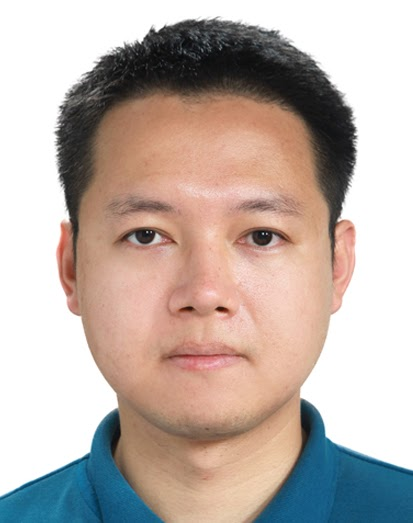
\includegraphics[width=1in,height=1.25in,clip,keepaspectratio]{authors/author2.jpg}}]{Cuong Manh Hoang}
is a Lecturer and AI Researcher with the Faculty of Information
Technology, Posts and Telecommunications Institute of Technology,
Hanoi, Vietnam. He received the B.S. degree in Robotics from Hanoi
University of Science and Technology, Vietnam, in 2017, the M.S.
degree in Robotics from the Deggendorf Institute of Technology,
Germany, in 2020, and the Ph.D. degree in Artificial Intelligence from
Seoul National University of Science and Technology, South Korea, in
2025. His research interests include computer vision, natural language
processing, vision-language understanding, and deep learning. He can be
contacted at cuonghm1@ptit.edu.vn.
\end{IEEEbiography}

\begin{IEEEbiography}[{
\includegraphics[width=1in,height=1.25in,clip,keepaspectratio]{authors/author3.jpg}}]{Nguyen Trung Hieu}
received the B.S. and M.Sc. degrees in electronics and
telecommunications, and the Ph.D. degree in electronics engineering,
from Posts and Telecommunications Institute of Technology (PTIT),
Hanoi, Vietnam, in 2006, 2010, and 2018, respectively. From 2006 to
the present, he has been a lecturer, Head of the Department of
Electronics and Computing Engineering, and Vice Dean of the Faculty of
Electronics Engineering 1 at PTIT, Hanoi, Vietnam. He is currently the
Dean of the Faculty of Electronics Engineering 1 at PTIT. His research
interests include coding theory, communication systems, IoT devices and
systems, and electronics design. Email: hieunt@ptit.edu.vn.
\end{IEEEbiography}

\begin{IEEEbiography}[{
\includegraphics[width=1in,height=1.25in,clip,keepaspectratio]{authors/author4.png}}]{Hoang Anh Pham}
received the B.S. degree in Electronics and Telecommunications and the
M.S. degree in Electronic Engineering from Hanoi University of Science
and Technology, Vietnam, in 2013 and 2015, respectively, and the Ph.D.
degree in Automation, Signal Processing, and Robotics from the
University of Toulon, France, in 2021. He conducted postdoctoral
research at the University of Toulon on cooperative control of
multi-robot systems under communication constraints. He is currently a
lecturer and researcher at the Posts and Telecommunications Institute
of Technology (PTIT), Vietnam. His research interests include control,
navigation, and localization for AUVs, UAVs, and multi-agent robotic
systems. Email: anhph@ptit.edu.vn.
\end{IEEEbiography}

\EOD
\end{document}
